% ============================================================
%  main.tex — AI Lab Paper (Sprint 1 skeleton)
%  Efficient Fine-Tuning of Small Open LLMs for Spanish
%  Sentiment Analysis
%
%  Template: IEEE Conference (IEEEtran)
%  Language:  English
%  Status:    Skeleton — all content sections are placeholders.
%             Results will be filled in Sprint 3.
%  Author:    Beltrán Sánchez Careaga
%  Created:   2026-06-04 by memoir-writer (claude-sonnet-4-6)
% ============================================================

\documentclass[conference]{IEEEtran}

% ---- Encoding and language ----
\usepackage[utf8]{inputenc}
% Spanish typesetting: es-tabla forces "Tabla" (not "Cuadro"); es-nodecimaldot
% keeps the decimal point inert in math so figures like $0.707$ and seed sets
% \{42, 43, 44\} render unchanged (no comma/point mixing).
\usepackage[spanish,es-tabla,es-nodecimaldot]{babel}
% IEEEtran's keyword label is English by default; localise it.
\renewcommand{\IEEEkeywordsname}{Palabras clave}

% ---- Mathematics ----
\usepackage{amsmath}
\usepackage{amssymb}

% ---- Graphics and figures ----
\usepackage{graphicx}
\graphicspath{{../results/figures/}}   % figures produced by ml-dev / qa-validator

% ---- Tables ----
\usepackage{booktabs}
\usepackage{multirow}

% ---- URLs and hyperlinks ----
\usepackage{url}
\usepackage{hyperref}
\hypersetup{
    colorlinks=true,
    linkcolor=black,
    citecolor=black,
    urlcolor=blue,
    pdftitle={Fine-tuning eficiente de LLM abiertos peque\~nos para el an\'alisis
              de sentimiento en espa\~nol: un estudio reproducible de LoRA/QLoRA
              bajo restricciones de c\'omputo de capa gratuita},
    pdfauthor={Beltr\'an S\'anchez Careaga}
}

% ---- Citations ----
% IEEEtran uses \cite{}; bibliography style set at end of file.

% ---- To-do notes (remove before final submission) ----
\usepackage[colorinlistoftodos, prependcaption]{todonotes}
% Usage: \todo{text}  or  \todo[inline]{text}
% To disable all todos for a clean build, replace the package line with:
%   \usepackage[disable]{todonotes}

% ---- Micro-typography ----
\usepackage{microtype}

% ============================================================
%  TITLE, AUTHORS, AFFILIATIONS
% ============================================================

\title{Fine-tuning eficiente de LLM abiertos pequeños para el análisis de sentimiento en español:\\
un estudio reproducible de LoRA/QLoRA bajo restricciones de cómputo de capa gratuita}

\author{
    \IEEEauthorblockN{Beltrán Sánchez Careaga}
    \IEEEauthorblockA{%
        \textit{Universidad Pontificia de Comillas -- ICAI}\\
        202216017@alu.comillas.edu
    }
}

% ============================================================
%  DOCUMENT
% ============================================================

\begin{document}

\maketitle

% ============================================================
%  ABSTRACT
% ============================================================

\begin{abstract}
El fine-tuning eficiente en parámetros (PEFT) con LoRA y QLoRA ha hecho
práctico adaptar grandes modelos de lenguaje a tareas específicas a una
fracción del coste del ajuste fino completo; sin embargo, varias preguntas
siguen abiertas para el texto de redes sociales en español: ¿a qué volumen de
datos supera el fine-tuning con LoRA al prompting few-shot del mismo modelo?;
¿pueden los LLM generativos pequeños con LoRA igualar a las líneas base de
codificadores establecidas en español en la frontera calidad-coste?; y
¿transfieren sin penalización los adaptadores LoRA entrenados en una variedad
dialectal del español a otras?
Abordamos las tres mediante un estudio empírico reproducible de Qwen3-1.7B y
Qwen3-4B con LoRA y QLoRA para el análisis de sentimiento de tuits en español
en tres clases, comparados con BETO y XLM-RoBERTa-base, en hardware GPU de
capa gratuita (objetivo de despliegue T4 16~GB).
Encontramos que el punto de cruce de prompting a fine-tuning depende del tamaño
del modelo: tan solo $n=7$ ejemplos etiquetados (el cruce se produce entre
$n=4$ y $n=7$) bastan para el modelo de 1.7B,
mientras que el modelo de 4B requiere aproximadamente $n=50$ debido a su mayor
suelo de prompting.
Con datos de entrenamiento completos, LoRA domina la frontera de Pareto
calidad-coste: Qwen3-4B LoRA alcanza macro-F1~$= 0.707$ y Qwen3-1.7B LoRA
alcanza $0.698$, superando a BETO ($0.661$) con ${\sim}9$--$17\times$ menos
parámetros entrenables (4B y 1.7B respectivamente).
QLoRA retiene el 97--99\% del F1 de LoRA con una VRAM pico 1.8--2.5$\times$
menor, lo que hace accesibles los modelos de 4B en hardware de consumo de
8~GB.
Un experimento de transferencia entre variedades sobre InterTASS~2018
(ibérico~ES, costarricense~CR, peruano~PE) revela una asimetría direccional: la
transferencia a CR y PE no tiene penalización, pero entrenar fuera del español
ibérico y apuntar a ES incurre en una pérdida consistente de macro-F1 de
0.031--0.039 puntos (2.6--4.6$\sigma$ de la variabilidad a nivel de semilla)
replicada en ambos tamaños de modelo.
Se publican todo el código, las configuraciones y las particiones de datos
preprocesadas para permitir la reproducibilidad completa en hardware de capa
gratuita.
\end{abstract}

% ============================================================
%  INDEX TERMS
% ============================================================

\begin{IEEEkeywords}
análisis de sentimiento, PLN en español, LoRA, QLoRA, PEFT,
fine-tuning de LLM, eficiencia de datos, aprendizaje con cómputo restringido,
transferencia dialectal
\end{IEEEkeywords}

% ============================================================
%  I. INTRODUCTION
% ============================================================

\section{Introducción}
\label{sec:introduction}

El análisis de sentimiento de texto de redes sociales en español se ha
convertido en una capacidad cada vez más importante para la monitorización de
la opinión pública, la inteligencia de marca y la investigación política.
Twitter y plataformas similares generan a diario millones de publicaciones en
español a lo largo de un amplio abanico de variedades dialectales y grupos
demográficos, lo que convierte la clasificación automática de sentimiento en
una tarea de gran valor pero técnicamente desafiante.
Al mismo tiempo, el coste de adaptar grandes modelos de lenguaje (LLM) a tareas
específicas ha sido históricamente prohibitivo: el ajuste fino completo de
modelos con miles de millones de parámetros requiere hardware GPU costoso y
grandes conjuntos de datos etiquetados que rara vez están disponibles en
dominios especializados.
Los métodos de fine-tuning eficiente en parámetros (PEFT) y, en particular,
LoRA~\cite{hu2021lora} y su variante con reconocimiento de cuantización
QLoRA~\cite{dettmers2023qlora}, han cambiado sustancialmente este panorama al
confinar la adaptación a un pequeño conjunto de matrices de bajo rango mientras
mantienen congelado el modelo base preentrenado, lo que permite un fine-tuning
eficaz con una fracción del presupuesto original de cómputo y
memoria~\cite{ding2023peftsurvey}.

A pesar de la rápida adopción de las técnicas PEFT, tres preguntas de relevancia
práctica siguen poco exploradas para el texto de redes sociales en español.
Primero, el grueso de la investigación PEFT existente se centra en el inglés o
se apoya en modelos con siete mil millones de parámetros o más, ejecutados en
hardware de nube premium (A100, H100).
El régimen de modelos generativos pequeños de pesos abiertos (1--4B parámetros)
en hardware GPU de capa gratuita (p.\ ej.\ T4 16~GB) ha recibido mucha menos
atención empírica, en particular para el español.
Segundo, aunque los enfoques basados en prompting ofrecen una alternativa
atractiva y de coste nulo al fine-tuning para modelos capaces, el punto de cruce
en el que el fine-tuning con LoRA empieza a superar al prompting few-shot del
mismo modelo no se ha medido de forma sistemática para el sentimiento de tuits
en español~\cite{mosbach2023fewshot,min2022rethinking}.
Del mismo modo, no existe un benchmark controlado que compare LLM generativos
pequeños con LoRA/QLoRA frente a modelos codificadores establecidos en
español---BETO~\cite{canete2020beto},
RoBERTuito~\cite{perez2022robertuito} y XLM-T~\cite{barbieri2022xlmt}---teniendo
en cuenta explícitamente el coste computacional en cada eje.
Tercero, aunque el español presenta una notable variación dialectal entre países,
no se ha caracterizado empíricamente si los adaptadores LoRA entrenados sobre una
variedad nacional transfieren sin penalización a otras---una cuestión con
implicaciones directas para decidir entre desplegar un único adaptador
panhispánico o adaptadores específicos por variedad.

Este artículo aborda estas tres cuestiones mediante un estudio empírico reproducible.
Nuestras contribuciones son:

\begin{itemize}
  \item \textbf{Punto de cruce de eficiencia de datos (Corte~A).} Aportamos la
    primera medición sistemática del punto de cruce de prompting few-shot a LoRA
    para el análisis de sentimiento de tuits en español, abarcando 11 tamaños de
    conjunto de entrenamiento y tres semillas aleatorias.
    Mostramos que este punto de cruce \emph{no} es un umbral universal: se
    produce con tan solo $n=7$ ejemplos etiquetados (entre
    $n=4$ y $n=7$) para Qwen3-1.7B (mejor prompting F1\,=\,0.560), pero se
    difiere hasta aproximadamente $n=50$ para
    Qwen3-4B (mejor prompting F1\,=\,0.652), porque el mayor suelo de prompting
    del modelo más grande exige más señal de fine-tuning para superarlo.

  \item \textbf{Benchmark de Pareto calidad-coste (Corte~B).} Evaluamos
    Qwen3-1.7B y Qwen3-4B con LoRA y QLoRA frente a BETO y
    XLM-RoBERTa-base (ambos con ajuste fino completo) en el conjunto de test
    Cardiff~ES, reportando la calidad de forma simultánea con los parámetros
    entrenables, la VRAM pico, el tiempo de entrenamiento y la latencia de
    inferencia.
    LoRA domina la frontera de Pareto: Qwen3-4B LoRA logra F1\,=\,0.707 y
    Qwen3-1.7B LoRA logra F1\,=\,0.698, superando al mejor codificador
    controlado (BETO~0.661) con aproximadamente $17\times$ menos parámetros
    entrenables.

  \item \textbf{Cuantificación del compromiso LoRA/QLoRA.} QLoRA retiene el
    97--99\% del macro-F1 de LoRA (0.681 y 0.701 frente a 0.698 y 0.707 para
    1.7B y 4B respectivamente) con una VRAM pico 1.8--2.5$\times$ menor (hasta
    4.93~GB y 6.79~GB), lo que hace accesibles los modelos de 4B en hardware de
    consumo de 8~GB.

  \item \textbf{Asimetría de transferencia dialectal (Corte~C).} Una matriz de
    transferencia entre variedades de $3\times3$ sobre InterTASS~2018~\cite{martinezcamara2018tass}
    (ibérico ES, costarricense CR, peruano PE) revela un resultado
    direccionalmente asimétrico: los adaptadores LoRA entrenados en cualquier
    variedad transfieren a CR y PE sin penalización, pero entrenar en CR o
    PE y evaluar en español ibérico incurre en una penalización consistente de
    macro-F1 de 0.031--0.039 puntos (2.6--4.6$\sigma$ de la variabilidad a nivel
    de semilla), que se replica en ambos tamaños de modelo.

  \item \textbf{Reproducibilidad en hardware de capa gratuita.} Se publican todo
    el código, las configuraciones de hiperparámetros y las particiones de datos
    preprocesadas, lo que permite la replicación en una única GPU T4 16~GB sin
    créditos de nube de pago.
\end{itemize}

El resto de este artículo se organiza como sigue:
la Sección~\ref{sec:related_work} revisa el trabajo relacionado sobre métodos
PEFT, análisis de sentimiento en español y transferencia dialectal;
la Sección~\ref{sec:methodology} describe los conjuntos de datos, los modelos y
el diseño experimental;
la Sección~\ref{sec:results} presenta los resultados de los Cortes~A, B y~C;
la Sección~\ref{sec:discussion} analiza las implicaciones prácticas y las
limitaciones; y la Sección~\ref{sec:conclusions} concluye con direcciones para
trabajo futuro.

% ============================================================
%  II. RELATED WORK
% ============================================================

\section{Trabajo relacionado}
\label{sec:related_work}

% ---- II-A. PEFT Methods ----
\subsection{Métodos de fine-tuning eficiente en parámetros}
\label{sec:related_peft}

El coste prohibitivo del ajuste fino completo de grandes modelos de lenguaje
preentrenados motivó una familia de métodos de fine-tuning eficiente en
parámetros (PEFT) que confinan la adaptación a un pequeño subconjunto de
parámetros mientras mantienen congelado el modelo base
preentrenado~\cite{ding2023peftsurvey}.
El enfoque fundacional de esta familia es el módulo adaptador introducido por
Houlsby et al.~\cite{houlsby2019adapters}, que inserta pequeñas capas de cuello
de botella entrenables entre los bloques transformer congelados; en el benchmark
GLUE, los adaptadores igualan el rendimiento del ajuste fino completo
actualizando menos del 4\% de los parámetros.

LoRA~\cite{hu2021lora} elimina el sobrecoste de los adaptadores en tiempo de
inferencia al reparametrizar las actualizaciones de pesos como el producto de
dos matrices de bajo rango ($\Delta W = AB$, con $r \ll d$).
Como las matrices de bajo rango se fusionan en los pesos base en tiempo de
inferencia, LoRA no introduce latencia adicional.
En el trabajo original, LoRA con rango $r=4$ iguala el ajuste fino completo de
GPT-3 (175B) en varios benchmarks mientras reduce los parámetros entrenables en
un factor de aproximadamente 10,000.

QLoRA~\cite{dettmers2023qlora} extiende LoRA con cuantización de los pesos base
en NF4 (Normal Float 4) y doble cuantización de las constantes de cuantización.
La combinación permite ajustar un modelo de 65B parámetros en una única GPU de
48\,GB con una pérdida de calidad insignificante, democratizando el acceso a
modelos muy grandes.
DoRA~\cite{liu2022dora} es una variante más reciente que descompone las
actualizaciones de pesos en componentes de magnitud y dirección, mejorando la
estabilidad del entrenamiento frente a LoRA estándar en varios benchmarks.
Todos estos métodos se unifican en la biblioteca PEFT~\cite{mangrulkar2022peft},
que proporciona una interfaz estandarizada para configuraciones de adaptadores,
LoRA y QLoRA.

\textbf{Hueco.}
La gran mayoría de los estudios PEFT se centran en el inglés, usan modelos con
siete mil millones de parámetros o más y se ejecutan en hardware de nube premium
(A100, H100).
El régimen de modelos generativos de pesos abiertos de 1--4B en hardware GPU de
capa gratuita (p.\ ej.\ T4 16\,GB) para lenguas distintas del inglés ha recibido
mucha menos atención empírica.
Nuestro trabajo llena este hueco aportando un benchmark controlado en ese régimen
para el español.

% ---- II-B. Sentiment Analysis in Spanish ----
\subsection{Análisis de sentimiento en español}
\label{sec:related_sentiment}

El análisis de sentimiento en español ha estado marcado por el desarrollo de
modelos solo de codificador, monolingües y multilingües, preentrenados en
grandes corpus en español.
BETO~\cite{canete2020beto}, un modelo BERT preentrenado en 3\,GB de texto en
español mediante enmascaramiento de palabra completa, estableció la primera
línea base monolingüe fuerte y sigue siendo un punto de referencia ampliamente
utilizado.
RoBERTuito~\cite{perez2022robertuito}, preentrenado en 500M de tuits en español
y empaquetado en la biblioteca \texttt{pysentimiento}, se especializa en texto
de redes sociales y alcanza un macro-F1 de aproximadamente 0.743 en el
benchmark TASS~2020~\cite{diazgaliano2020tass}---el corpus canónico de
evaluación de sentimiento en español producido por la comunidad SEPLN, que
cubre múltiples variedades dialectales a través de su pista InterTASS.
MarIA~\cite{gutierrezfandino2022maria} es una familia de modelos RoBERTa en
español (base y grande) preentrenados en un corpus web en español de 570\,GB
por la Biblioteca Nacional de España; su variante grande supera a BETO en la
mayoría de los benchmarks de PLN en español.

En el lado multilingüe, XLM-RoBERTa~\cite{conneau2020xlmr} proporciona un
codificador masivamente multilingüe (100 lenguas, 278M de parámetros) que
compite con los modelos monolingües en tareas en español sin requerir
preentrenamiento específico de la lengua.
XLM-T~\cite{barbieri2022xlmt} extiende esta línea al continuar el
preentrenamiento de XLM-RoBERTa en un gran corpus multilingüe de Twitter
(198M de tuits) y publicar el conjunto de datos multilingüe de sentimiento de
tuits de Cardiff~NLP---el mismo conjunto de datos utilizado en este estudio.

\textbf{Hueco.}
Todos los sistemas anteriores son modelos solo de codificador evaluados con
ajuste fino completo, y la calidad se reporta de forma aislada del coste
computacional.
Ningún benchmark controlado compara simultáneamente LLM generativos pequeños de
pesos abiertos con LoRA/QLoRA frente a estos codificadores establecidos
reportando calidad y coste (parámetros entrenables, VRAM, tiempo de
entrenamiento, latencia de inferencia) en el mismo conjunto de test.
El Corte~B de este artículo proporciona exactamente ese benchmark.

% ---- II-C. Few-Shot Prompting vs.\ Fine-Tuning ----
\subsection{Prompting few-shot frente al fine-tuning}
\label{sec:related_dialectal}

La aparición de grandes modelos de lenguaje con fuertes capacidades de
aprendizaje en contexto (ICL) ha reabierto la cuestión de cuándo el fine-tuning
con datos etiquetados es preferible al prompting few-shot.
Mosbach et al.~\cite{mosbach2023fewshot} presentan una comparación rigurosa y
directa entre el fine-tuning few-shot y el ICL a lo largo de un amplio conjunto
de benchmarks de clasificación.
Su hallazgo principal es que el fine-tuning es consistentemente superior cuando
se dispone de $n \geq 64$ ejemplos etiquetados, pero que el ICL es
competitivo---y a veces mejor---en el régimen de muy pocos datos ($n \leq 16$).
Min et al.~\cite{min2022rethinking} cuestionan la interpretación convencional
del ICL: mediante experimentos de ablación, muestran que el papel de las
demostraciones en contexto es principalmente transmitir el formato de salida y
el espacio de etiquetas, en lugar de enseñar el mapeo correcto entre entrada y
salida.
Esto implica que el techo de calidad del prompting está gobernado principalmente
por el conocimiento preentrenado del modelo, no por los ejemplos concretos
mostrados.

Estos dos hallazgos en conjunto tienen una implicación concreta para el punto de
cruce que medimos en el Corte~A: si el techo de calidad del prompting lo
determina la propia capacidad del modelo, entonces un modelo base más fuerte
tendrá un suelo de prompting más alto, lo que exige más señal etiquetada de
fine-tuning para superarlo.
Esto es precisamente lo que observamos: Qwen3-1.7B, con un mejor F1 de prompting
de 0.560, es superado por LoRA en $n=7$, mientras que Qwen3-4B, cuyo suelo de
prompting alcanza 0.652, requiere aproximadamente $n=50$ ejemplos antes de que
el fine-tuning se imponga.

\textbf{Hueco.}
Ninguno de los dos estudios mide el punto de cruce de forma sistemática para el
análisis de sentimiento en español, a lo largo de múltiples tamaños de conjunto
de entrenamiento, múltiples semillas independientes y subconjuntos
disjuntos---el diseño que adoptamos en el Corte~A para garantizar que nuestras
desviaciones típicas reflejen una varianza genuina de muestreo de datos.

% ---- II-D. PEFT for Clinical Spanish (Differentiator) ----
\subsection{PEFT para texto clínico en español}
\label{sec:related_clinical}

Los métodos PEFT también han encontrado aplicación en el PLN clínico en español.
La tarea compartida DisTEMIST~\cite{mirandaescalada2023distemist} evaluó la
detección y normalización de menciones de enfermedades en notas clínicas en
español (corpus SPACCC, Hospital Cl\'{i}nic Barcelona); los sistemas con mejor
rendimiento emplearon fine-tuning basado en adaptadores sobre BETO y MarIA en
hardware biomédico dedicado, demostrando que el PEFT puede igualar o superar el
ajuste fino completo incluso en dominios especializados de bajos recursos.

Nuestro trabajo difiere de esta dirección clínica en cuatro aspectos:
(1)~\textbf{tarea} (clasificación de sentimiento frente a NER
clínico/codificación de diagnósticos); (2)~\textbf{dominio} (texto de redes
sociales de Twitter frente a notas clínicas hospitalarias); (3)~\textbf{familia
de modelos} (LLM generativos solo de decodificador frente a modelos solo de
codificador); y (4)~\textbf{hardware} (T4 16\,GB de capa gratuita frente a
hardware premium A100).

\medskip
\noindent
Este artículo ocupa la intersección de tres líneas de investigación que hasta
ahora han permanecido separadas: PEFT aplicado a LLM generativos pequeños de
pesos abiertos (1--4B), análisis de sentimiento de redes sociales en español, y
benchmarking consciente del coste bajo restricciones de cómputo de capa
gratuita.
En concreto, ningún trabajo existente proporciona una comparación controlada del
fine-tuning con LoRA/QLoRA frente a modelos codificadores establecidos en
español que mida simultáneamente la calidad y las cuatro dimensiones de coste
(parámetros entrenables, VRAM, tiempo de entrenamiento, latencia de inferencia)
en un conjunto de test reservado común---ni ningún trabajo caracteriza el punto
de cruce de prompting a fine-tuning para el sentimiento de tuits en español a lo
largo de múltiples tamaños de entrenamiento y semillas independientes.
Las contribuciones de este artículo llenan ese hueco.

% ============================================================
%  III. METHODOLOGY
% ============================================================

\section{Metodología}
\label{sec:methodology}

% ---- III-A. Dataset ----
\subsection{Conjunto de datos}
\label{sec:methodology_dataset}

Usamos el subconjunto en español del corpus \textbf{Cardiff NLP Tweet Sentiment
Multilingual}~\cite{barbieri2022xlmt}, publicado bajo CC~BY~4.0 y disponible en
Hugging Face (\texttt{cardiffnlp/tweet\_sentiment\_multilingual}).
El corpus contiene tuits en español anotados con tres etiquetas de sentimiento:
\textit{positivo}, \textit{negativo} y \textit{neutral}.
Tamaños de las particiones: \textbf{1{,}839 ejemplos de entrenamiento}
(613 por clase), \textbf{324 ejemplos de validación} (108 por clase) y
\textbf{870 ejemplos de test} (290 por clase).
La distribución de clases está perfectamente balanceada en todas las
particiones.

Para el estudio de eficiencia de datos (Corte~A) construimos submuestras de
entrenamiento estratificadas por clase en $n \in \{4,\, 7,\, 10,\, 16,\, 25,\,
50,\, 100,\, 250,\, 500,\, 1{,}000\}$ más el conjunto completo (1,839 ejemplos),
abarcando 11 tamaños de entrenamiento.
De forma crítica, cada una de las tres semillas aleatorias $\{42, 43, 44\}$
extrae una submuestra estratificada \emph{independiente}, de modo que los
ejemplos usados para una semilla son disjuntos de los usados para otra en cada
tamaño (p.\ ej.\ 0 ejemplos compartidos en $n=4$, 0 en $n=10$).
La estratificación garantiza que las tres clases estén representadas en cada
celda; en $n=4$ esto da negativo=2, neutral=1, positivo=1.
Los tamaños más pequeños, $n=4$ y $n=7$, se añadieron específicamente para
localizar el punto de cruce entre LoRA y prompting por debajo de $n=10$.
(Implementación: \texttt{scripts/build\_fraction\_subsets.py}.)

Seleccionamos este conjunto de datos por tres razones: (1)~acceso abierto bajo
CC~BY~4.0, que no requiere licencia institucional; (2)~particiones fijas y
predefinidas que eliminan la varianza inducida por la partición y permiten la
comparación entre estudios; y (3)~amplia adopción en la
literatura~\cite{barbieri2022xlmt}.
No se redistribuye el texto bruto de los tuits; el repositorio proporciona
scripts de descarga y preprocesamiento.
\textbf{InterTASS 2018 (solo Corte~C).}
El Corte~C utiliza la pista dialectal InterTASS 2018~\cite{martinezcamara2018tass},
un subconjunto de la serie más amplia de evaluación de sentimiento TASS
organizada por SEPLN.
Se incluyen tres variedades nacionales: español ibérico (ES), español
costarricense (CR) y español peruano (PE).
Tras descartar la etiqueta de polaridad \textit{NONE} (instancias sin objetivo
presente que contaminarían el esquema de polaridad de tres clases), los
conjuntos utilizables contienen 738 / 539 / 541 ejemplos de entrenamiento para
ES, CR y PE respectivamente.
Una partición reservada estratificada del 15\% de cada conjunto de entrenamiento
se reserva para la selección de checkpoint; la evaluación usa las particiones de
desarrollo de InterTASS 2018 (444~ES / 242~CR / 262~PE).
Las etiquetas de oro del test de InterTASS 2018 se distribuyen como un fichero
\texttt{.qrel} que estaba inaccesible (HTTP~404) en el momento de redactar este
trabajo; por tanto, la evaluación se realiza exclusivamente sobre las
particiones de desarrollo (véase la Sección~\ref{sec:results_C} para la
declaración metodológica completa).
El corpus CardiffNLP descrito arriba \emph{no} se usa en el Corte~C; los dos
conjuntos de datos se evalúan de forma completamente independiente.

% ---- III-B. Models ----
\subsection{Modelos}
\label{sec:methodology_models}

\subsubsection*{Líneas base}
\label{sec:methodology_baselines}

\textbf{Línea base léxica.}
Un vectorizador TF-IDF ($n$-gramas de caracteres, 2--4) combinado con un
clasificador de regresión logística proporciona el suelo de coste de la frontera
calidad-coste.
No requiere GPU y alcanza un macro-F1 de \textbf{0.566} en el conjunto de test
Cardiff~ES.

\textbf{Líneas base de codificadores (controladas, en la frontera de Pareto).}
Se hace fine-tuning de dos modelos solo de codificador sobre el conjunto de
entrenamiento Cardiff~ES (semilla~42, 3 épocas, lr~=~2$\times$10$^{-5}$, tamaño
de lote~16):
(1)~\textbf{BETO}~\cite{canete2020beto}
(\texttt{dccuchile/\allowbreak bert-base-spanish-wwm-cased}), un modelo BERT preentrenado en
corpus en español; y
(2)~\textbf{XLM-RoBERTa-base}~\cite{conneau2020xlmr}, un modelo RoBERTa
masivamente multilingüe.
Ambos se entrenan a partir de pesos preentrenados disponibles públicamente sin
fine-tuning previo en Cardiff~ES, lo que garantiza una comparación controlada y
justa con los modelos generativos en la frontera de Pareto (Corte~B).
En el conjunto de test Cardiff~ES alcanzan un macro-F1 de \textbf{0.661} (BETO) y
\textbf{0.646} (XLM-RoBERTa-base), ambos claramente por encima del suelo léxico
(Tabla~\ref{tab:baselines}).
El modelo \texttt{cardiffnlp/\allowbreak twitter-\allowbreak xlm-roberta-\allowbreak base-sentiment-\allowbreak multilingual} se
excluyó porque se le había hecho fine-tuning sobre el mismo conjunto de datos
usado para nuestra partición de test, lo que constituye una fuga de distribución.

\textbf{Referencia lista para usar (fuera de dominio, no en la frontera de Pareto).}
\texttt{pysentimiento/\allowbreak robertuito-sentiment-analysis}~\cite{perez2022robertuito}
se evalúa en modo zero-shot sobre la partición de test Cardiff~ES.
A este modelo se le hizo fine-tuning sobre TASS~2020, un corpus de sentimiento en
español distinto, por lo que \emph{no} se sitúa en la frontera de Pareto; sirve
como referencia contextual de transferencia fuera de dominio.

\textbf{Línea base de prompting.}
Qwen3-1.7B~\cite{qwen3technicalreport2025} se evalúa en modos zero-shot y
few-shot ($k \in \{4,\, 8,\, 16\}$ ejemplos en contexto).
El protocolo está congelado en \texttt{configs/prompting\_protocol.yaml}: se
consulta el modelo a través de su plantilla de chat con el modo de pensamiento
desactivado, un prompt de sistema directivo y los ejemplos few-shot
representados como turnos alternos de usuario/asistente (selección aleatoria
estratificada, semilla~42); se asigna la etiqueta de reserva (\textit{neutral})
cuando no se devuelve ninguna etiqueta interpretable, y la tasa de reserva se
registra por ejecución como indicador de calidad.
Este mismo protocolo se aplica a Qwen3-4B en el Sprint~3.
En el conjunto de test Cardiff~ES, Qwen3-1.7B alcanza una exactitud de 0.508
(macro-F1 0.471) en zero-shot y hasta 0.561 (macro-F1 0.560) con $k=8$ ejemplos
few-shot, con una tasa de reserva igual o inferior al 1.4\,\% en todas las
configuraciones.
Estos puntos de prompting se sitúan entre las líneas base léxica y de
codificadores y se retoman frente al fine-tuning con LoRA/QLoRA en el Corte~A.

\subsubsection*{LLM generativos con LoRA/QLoRA}
Los principales modelos experimentales son Qwen3-1.7B y
Qwen3-4B~\cite{qwen3technicalreport2025} (licencia Apache~2.0), elegidos por su
fuerte soporte multilingüe y su compatibilidad con QLoRA en 16~GB de VRAM.
Los detalles del fine-tuning se describen en la
Sección~\ref{sec:methodology_setup}.

% ---- III-C. Fine-Tuning Setup ----
\subsection{Configuración del fine-tuning}
\label{sec:methodology_setup}

\subsubsection*{Diseño experimental}

La rejilla se organiza en tres cortes complementarios
(generados por \texttt{scripts/gen\_sprint3\_grid.py}):

\textbf{Corte~A (eficiencia de datos / punto de cruce).}
LoRA $\times$ \{Qwen3-1.7B, Qwen3-4B\} $\times$ 11 tamaños de entrenamiento
$\times$ 3 semillas $= 66$ celdas.
Cada celda se evalúa sobre el conjunto de test completo de 870 ejemplos.
Los resultados se comparan con el prompting zero-shot y few-shot de los mismos
dos modelos, estableciendo el punto de cruce en el que el fine-tuning supera al
aprendizaje en contexto.

\textbf{Corte~B (calidad--coste / Pareto).}
Con datos de entrenamiento completos (1,839 ejemplos) y una única semilla (42),
comparamos LoRA, QLoRA y ajuste fino completo (tres comprobaciones puntuales)
junto a las líneas base de codificadores (BETO, XLM-RoBERTa) y la referencia de
prompting.
El Corte~B reporta calidad frente a coste en cuatro dimensiones: parámetros
entrenables, VRAM pico, tiempo de entrenamiento y latencia de inferencia.
El diseño de una sola semilla se justifica por la varianza de semilla
insignificante observada para Qwen3-1.7B con datos completos
(desv.\ típica $\approx \pm0.006$ F1).

\textbf{Corte~C (transferencia dialectal).}
LoRA $\times$ \{Qwen3-1.7B, Qwen3-4B\} $\times$ 3~variedades de origen $\times$
3~variedades objetivo $\times$ 3~semillas $=$ 54 celdas.
Cada celda entrena sobre la partición de entrenamiento completa de
InterTASS~2018 de la variedad de origen (tras eliminar NONE) y evalúa sobre la
partición de desarrollo de la variedad objetivo.
Los hiperparámetros de LoRA son idénticos a los del Corte~B; se usan el mismo
arnés generativo y el mismo protocolo de selección de checkpoint.

\subsubsection*{Configuración de LoRA}

Los adaptadores LoRA~\cite{hu2021lora} se aplican con rango $r=16$,
factor de escala $\alpha=32$, dropout $p=0.05$ y módulos objetivo
\texttt{\{q,\,k,\,v,\,o\}\_proj} (solo las proyecciones de atención),
bias \texttt{none}, tipo de tarea \texttt{CAUSAL\_LM}.
Estos valores se mantienen fijos en todas las celdas LoRA y QLoRA.

\subsubsection*{Configuración de QLoRA}

Para QLoRA~\cite{dettmers2023qlora}, el modelo base se carga en precisión de
4 bits usando la \texttt{BitsAndBytesConfig} definida en
\texttt{src/models/lora\_finetune.py}: tipo de cuantización NF4
(\texttt{bnb\_4bit\_quant\_type="nf4"}), doble cuantización activada
(\texttt{bnb\_4bit\_use\_double\_quant=True}) y bfloat16 como dtype de cómputo
(\texttt{bnb\_4bit\_compute\_dtype=torch.bfloat16}).
Tras la carga, se aplica \texttt{prepare\_\allowbreak model\_\allowbreak for\_\allowbreak kbit\_\allowbreak training} y se activa
el checkpointing de gradientes, manteniendo el uso de VRAM holgadamente dentro
del objetivo de despliegue de 16~GB de hardware de capa gratuita.
A continuación se aplica la misma configuración de LoRA anterior sobre el modelo
base cuantizado.

\subsubsection*{Configuración del ajuste fino completo}

Para la comprobación puntual de ajuste fino completo (Corte~B), todos los pesos
del modelo se hacen entrenables y la tasa de aprendizaje se reduce a
$1 \times 10^{-5}$ (frente a $2 \times 10^{-4}$ para LoRA/QLoRA) con un mínimo de
60 pasos.

\subsubsection*{Planificación del entrenamiento}

Todas las celdas LoRA y QLoRA comparten la siguiente planificación:
tasa de aprendizaje $2 \times 10^{-4}$, planificador coseno con ratio de
calentamiento 0.1, 5 épocas, tamaño de lote 8, acumulación de gradientes 1,
longitud máxima de secuencia 256, precisión bf16.
Para asegurar que las fracciones de entrenamiento muy pequeñas no queden
infraentrenadas, el número de pasos de optimización se acota inferiormente a:
$\text{max\_steps} = \max\!\left(80,\ 5 \cdot \lceil n / 8 \rceil\right)$,
de modo que incluso la celda de cuatro ejemplos recibe al menos 80 pasos de
actualización.
El macro-F1 de validación se evalúa 4 veces durante el entrenamiento (espaciado
uniformemente a lo largo de \texttt{max\_steps}).

\subsubsection*{Selección de modelo y objetivo SFT}

Se selecciona como modelo final el checkpoint con el \emph{mayor macro-F1 de
validación}, no el último paso (implementado mediante
\texttt{BestValF1Callback} en \texttt{src/models/lora\_finetune.py}).
El objetivo SFT enmascara los tokens del prompt con $-100$; solo el token de
etiqueta (uno de \textit{negative}, \textit{neutral}, \textit{positive}) y el
token EOS contribuyen a la pérdida de entropía cruzada.
La estructura del prompt (prompt de sistema, señal de respuesta, plantilla de
chat, modo de pensamiento desactivado) es idéntica a la de la línea base de
prompting, lo que garantiza que la única variable entre prompting y fine-tuning
sea la presencia de pesos actualizados.

\subsubsection*{Marco de trabajo y hardware}

Los experimentos usan HuggingFace Transformers con la biblioteca
PEFT~\cite{mangrulkar2022peft}.
La rejilla PEFT y todas las evaluaciones se ejecutaron en GPU NVIDIA H200 (dos
carriles paralelos: Qwen3-1.7B en el carril~A, Qwen3-4B en el carril~B).
La VRAM pico de GPU se registra por celda mediante
\texttt{torch.cuda.max\_memory\_allocated()} para validar la viabilidad en
hardware de capa gratuita de 16~GB, que es el objetivo de despliegue del artículo
(según el título); las cifras exactas de VRAM se reportan en las tablas de
resultados.

\subsubsection*{Política de semillas}

El Corte~A usa tres semillas independientes $\{42, 43, 44\}$; se reportan la
media y la desviación típica sobre las tres semillas.
El Corte~B usa una única semilla (42) porque la varianza de semilla con datos
completos es insignificante (desv.\ típica de LoRA con datos completos para
Qwen3-1.7B $\approx \pm0.006$ F1 macro).
La siembra global de todas las ejecuciones se realiza mediante
\texttt{src/utils/seed.py}~(\texttt{set\_seed}).

% ---- III-D. Evaluation Protocol ----
\subsection{Protocolo de evaluación}
\label{sec:methodology_evaluation}

La métrica principal de calidad es el \textbf{macro-F1} promediado sobre las
tres clases (positivo, negativo, neutral), que trata todas las clases por igual
y es robusto frente a las diferencias de dificultad entre clases.
Para las celdas del Corte~A, se reportan la media y la desviación típica sobre
tres semillas aleatorias independientes $\{42, 43, 44\}$.
Para las celdas del Corte~B (comprobaciones puntuales con datos completos) y las
líneas base de codificadores, se usa una única semilla (42); la justificación se
da en la Sección~\ref{sec:methodology_setup}.

Registramos cuatro \textbf{métricas de coste} para cada celda experimental:
(1)~número de parámetros entrenables;
(2)~VRAM pico de GPU en GB, medida mediante
\texttt{torch.cuda.max\_memory\_allocated()};
(3)~tiempo de ejecución del entrenamiento en segundos; y
(4)~latencia de inferencia en ms por ejemplo, promediada sobre el conjunto de
test.

Todas las evaluaciones usan la misma partición de test Cardiff~ES predefinida
(870 ejemplos, balanceada), lo que garantiza la comparabilidad directa entre
modelos y métodos.
La selección de hiperparámetros se realiza exclusivamente sobre la partición de
validación de 324 ejemplos; la partición de test se accede una sola vez, en la
evaluación final, sin fuga de datos.

Los modelos generativos con fine-tuning reutilizan el \emph{mismo} arnés
generativo que la línea base de prompting (modo zero-shot, $k=0$): el modelo
genera una respuesta, se extrae la primera palabra de etiqueta coincidente y se
aplica la etiqueta de reserva (\textit{neutral}) cuando no se encuentra ninguna
etiqueta interpretable.
La tasa de reserva se registra por celda experimental como indicador de calidad
adicional.
Este arnés unificado, implementado mediante \texttt{PromptingBaseline} en
\texttt{src/models/prompting.py}, garantiza que las diferencias de calidad entre
las variantes de prompting y de fine-tuning no puedan atribuirse a diferencias en
el protocolo de evaluación.

% ============================================================
%  IV. EXPERIMENTS AND RESULTS
% ============================================================

\section{Experimentos y resultados}
\label{sec:results}

Presentamos los resultados de cuatro líneas experimentales: los puntos de
referencia no generativos (Sección~\ref{sec:results_baselines}), el punto de
cruce de eficiencia de datos (Sección~\ref{sec:results_A}), el benchmark
calidad-coste con datos completos (Sección~\ref{sec:results_B}) y el análisis de
transferencia dialectal (Sección~\ref{sec:results_C}).

\subsection{Puntos de referencia de las líneas base}
\label{sec:results_baselines}

La Tabla~\ref{tab:baselines} reporta los puntos de referencia no generativos que
anclan la frontera calidad-coste, todos evaluados sobre la misma partición de
test reservada Cardiff~ES (870 ejemplos, semilla~42).
Los dos codificadores controlados (BETO, XLM-RoBERTa-base) reciben ajuste fino
completo durante 3~épocas y se sitúan en la frontera de Pareto; el modelo léxico
TF-IDF\,+\,LR proporciona el suelo de coste; y
\texttt{pysentimiento/robertuito} es una referencia fuera de dominio (con
fine-tuning sobre TASS~2020, evaluada en zero-shot) que \emph{no} se sitúa en la
frontera.
Los resultados generativos de prompting y LoRA/QLoRA se reportan en las
Secciones~\ref{sec:results_A}--\ref{sec:results_B}.

\begin{table}[t]
  \centering
  \caption{Resultados de las líneas base en el conjunto de test Cardiff~ES
    (semilla~42). A los codificadores se les hace ajuste fino completo durante
    3~épocas (lr~$=2\times10^{-5}$, lote~16).
    RoBERTuito es una referencia fuera de dominio, no en la frontera de Pareto.}
  \label{tab:baselines}
  \small
  \resizebox{\columnwidth}{!}{%
  \begin{tabular}{@{}llrr@{}}
    \toprule
    Modelo & Método & Macro-F1 & Exac. \\
    \midrule
    TF-IDF\,+\,LR            & léxico (sin GPU)        & 0.566 & 0.569 \\
    BETO                     & FT completo (3~ép.)     & \textbf{0.661} & 0.663 \\
    XLM-RoBERTa-base         & FT completo (3~ép.)     & 0.646 & 0.660 \\
    \midrule
    RoBERTuito\,$^{\dagger}$ & listo para usar (0-shot) & 0.758 & 0.761 \\
    \bottomrule
  \end{tabular}}
  \\[2pt]
  {\footnotesize $^{\dagger}$Referencia fuera de dominio (TASS~2020), excluida de la frontera de Pareto.}
\end{table}

% ---- IV-A. Cut A: Data-efficiency crossover ----
\subsection{Corte A: punto de cruce de eficiencia de datos}
\label{sec:results_A}

\subsubsection*{Protocolo experimental}
Los subconjuntos de entrenamiento se extraen por muestreo \emph{estratificado}
por fracciones de modo que las tres clases de sentimiento estén representadas en
cada celda: en $n=4$ la partición es negativo\,=\,2, neutral\,=\,1,
positivo\,=\,1; en $n=10$ es de 3--4 por clase.
El Corte~A usa tres semillas $\{42,43,44\}$, y cada semilla extrae un
subconjunto \emph{independiente y disjunto} de los datos de entrenamiento
(0 de 4 ejemplos se comparten en $n=4$; 0 de 10 en $n=10$), de modo que las
desviaciones típicas reportadas reflejan la varianza de muestreo de datos, no
solo el ruido de inicialización de pesos.
Los mejores checkpoints se seleccionan por el macro-F1 de validación; la
evaluación final usa el conjunto de test completo Cardiff~ES de 870 ejemplos con
el mismo arnés generativo empleado para las líneas base de prompting
(parseo\,+\,reserva neutral; tasa de reserva $\approx 0$ para todos los modelos
con fine-tuning).
Los hiperparámetros de LoRA se mantienen fijos en todas las celdas: $r=16$,
$\alpha=32$, dropout~$= 0.05$, módulos objetivo $\{q,k,v,o\}$\_proj,
lr~$=2\times10^{-4}$, 5~épocas con un mínimo de 80~pasos de gradiente.

\subsubsection*{Resultados}

La Tabla~\ref{tab:cutA} y la Figura~\ref{fig:cutA} resumen el macro-F1 en función
del tamaño del conjunto de entrenamiento $n$ para Qwen3-1.7B y Qwen3-4B con
fine-tuning LoRA (media~$\pm$ desv.\ típica sobre tres semillas independientes),
junto con las líneas base de prompting independientes de N.

El hallazgo más importante es que el \textbf{punto de cruce en el que LoRA supera
al mejor resultado de prompting se desplaza marcadamente hacia la derecha a
medida que crece la capacidad del modelo}.
Para Qwen3-1.7B, cuyo mejor resultado de prompting es 0.560 (k\,=\,8 few-shot),
LoRA ya supera este listón en $n=7$ ($0.590 \pm 0.063$), tras haber estado por
debajo en $n=4$ ($0.539 \pm 0.010$).
El modelo de 1.7B necesita, por tanto, menos de diez ejemplos etiquetados para
justificar el fine-tuning frente al aprendizaje en contexto.

Para Qwen3-4B el panorama es fundamentalmente distinto.
Su F1 zero-shot ya es 0.633---por encima del mejor resultado de prompting de
1.7B---y su mejor puntuación de prompting alcanza 0.652 ($k=4$).
El fine-tuning en $n=7$ produce solo $0.645 \pm 0.038$, todavía por debajo de
este listón, e incluso $n=25$ ($0.645 \pm 0.037$) queda en él o justo por debajo.
El punto de cruce no se cruza con firmeza hasta aproximadamente $n=50$
($0.666 \pm 0.034$), lo que representa aproximadamente un orden de magnitud más
de datos etiquetados que los requeridos por el modelo más pequeño.
El mecanismo es sencillo: un suelo de prompting más fuerte requiere más señal de
fine-tuning para superarlo.
Este desplazamiento dependiente del tamaño---no un único umbral universal---es el
hallazgo empírico central del Corte~A.

Más allá del punto de cruce, ambos modelos mejoran de forma sostenida con los
datos, alcanzando $0.683 \pm 0.015$ (1.7B) y $0.687 \pm 0.009$ (4B) en $n=500$, y
$0.698 \pm 0.006$ (1.7B) y $0.707 \pm 0.022$ (4B) con datos completos
($n=1{,}839$).
Las ganancias se vuelven sublineales por encima de $n\approx250$, lo que sugiere
rendimientos decrecientes en este régimen; sin embargo, el beneficio marginal de
datos adicionales sigue siendo estadísticamente discernible hasta $n=1{,}000$.
La gran varianza en $n=4$ para Qwen3-4B ($\pm0.089$) refleja la sensibilidad
extrema del modelo al adaptarse a partir de solo uno o dos ejemplos por clase;
esta varianza se contrae sustancialmente hacia $n=25$.

\begin{table}[t]
  \centering
  \caption{Corte~A: macro-F1 de LoRA (media\,$\pm$\,desv.\ típica sobre 3
    semillas \{42,43,44\}) en el conjunto de test Cardiff~ES ($n=870$) en
    función del tamaño del conjunto de entrenamiento.
    Las filas de prompting (abajo) son resultados independientes de N de una
    sola semilla (42) y se incluyen únicamente como referencia del punto de
    cruce.}
  \label{tab:cutA}
  \small
  \begin{tabular}{@{}lrr@{}}
    \toprule
    $n$ & Qwen3-1.7B F1 & Qwen3-4B F1 \\
    \midrule
    4    & $0.539 \pm 0.010$ & $0.522 \pm 0.089$ \\
    7    & $0.590 \pm 0.063$ & $0.645 \pm 0.038$ \\
    10   & $0.598 \pm 0.035$ & $0.638 \pm 0.013$ \\
    16   & $0.622 \pm 0.026$ & $0.641 \pm 0.068$ \\
    25   & $0.654 \pm 0.023$ & $0.645 \pm 0.037$ \\
    50   & $0.632 \pm 0.030$ & $0.666 \pm 0.034$ \\
    100  & $0.645 \pm 0.024$ & $0.687 \pm 0.014$ \\
    250  & $0.657 \pm 0.011$ & $0.698 \pm 0.002$ \\
    500  & $0.683 \pm 0.015$ & $0.687 \pm 0.009$ \\
    1000 & $0.685 \pm 0.005$ & $0.698 \pm 0.007$ \\
    completo & $0.698 \pm 0.006$ & $0.707 \pm 0.022$ \\
    \midrule
    \multicolumn{3}{@{}l}{\textit{Líneas base de prompting (independientes de N, semilla 42)}} \\
    0-shot  & 0.471 & 0.633 \\
    k=4     & 0.544 & \textbf{0.652} \\
    k=8     & \textbf{0.560} & 0.590 \\
    k=16    & 0.540 & 0.631 \\
    \bottomrule
  \end{tabular}
\end{table}

\begin{figure}[t]
  \centering
  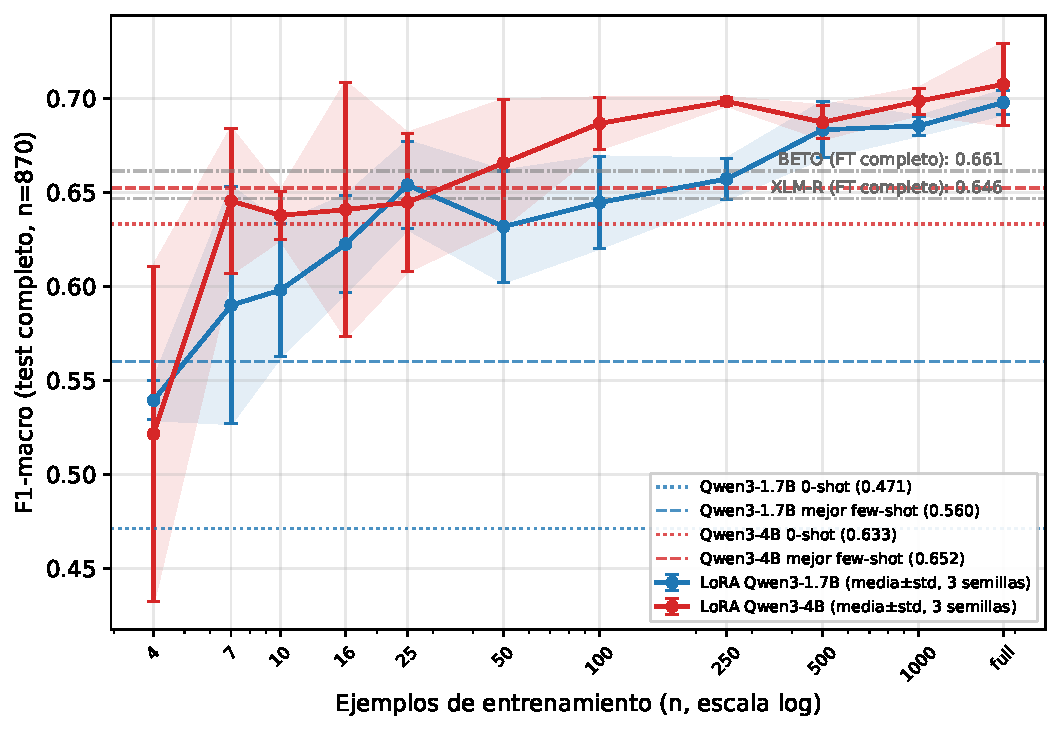
\includegraphics[width=\columnwidth]{figA_f1_vs_n_paper}
  \caption{Macro-F1 frente al tamaño del conjunto de entrenamiento $n$
    (escala log) para Qwen3-1.7B y Qwen3-4B con fine-tuning LoRA (bandas de
    media\,$\pm$\,desv.\ típica sobre 3 semillas).  Las líneas discontinuas
    horizontales muestran el mejor F1 de prompting few-shot de cada modelo y los
    anclajes de codificadores controlados (BETO~0.661, XLM-R~0.646).  El cruce de
    prompting a LoRA se produce entre $n=4$ y $n=7$ para el modelo de 1.7B, pero
    se difiere hasta aproximadamente $n=50$ para el modelo de 4B, porque el suelo
    de prompting del modelo más grande es sustancialmente más fuerte (mejor
    few-shot 0.652 frente a 0.560).}
  \label{fig:cutA}
\end{figure}

% ---- IV-B. Cut B: Generative LLMs vs. Encoders ----
\subsection{Corte B: LLM generativos frente a codificadores establecidos}
\label{sec:results_B}

\subsubsection*{Protocolo experimental}
El Corte~B compara los métodos con datos completos con una única semilla (42),
lo que se justifica porque la varianza de semilla es insignificante a esta
escala: la ejecución de LoRA con datos completos de Qwen3-1.7B tiene una
desviación típica de solo $\pm0.006$ entre tres semillas
(Tabla~\ref{tab:cutA}).  La excepción es LoRA con datos completos para ambos
modelos, para los que se ejecutaron tres semillas y los resultados se reportan
como media\,$\pm$\,desv.\ típica.
El conjunto de evaluación y el arnés generativo son idénticos a los del Corte~A.
El ajuste fino completo de Qwen3-1.7B usa lr\,$= 1\times10^{-5}$ para evitar el
olvido catastrófico; todos los demás hiperparámetros coinciden con la
configuración de LoRA.

\subsubsection*{Resultados}

La Tabla~\ref{tab:cutB} reporta el macro-F1 junto con las cuatro dimensiones de
coste (parámetros entrenables, VRAM pico, tiempo de ejecución del entrenamiento
y latencia de inferencia) para cada combinación (método, modelo).
Los anclajes de codificadores de la Tabla~\ref{tab:baselines} se incluyen como
referencia.
La Figura~\ref{fig:cutB} visualiza la vista de Pareto calidad frente a parámetros
entrenables, y la Figura~\ref{fig:cutB_cost} la complementa incorporando la VRAM
pico y la latencia de inferencia.

\textbf{LoRA domina la frontera de Pareto.}
Ambas configuraciones LoRA superan al mejor codificador controlado
(BETO~0.661) entrenando solo 6--12\,M de parámetros.
Qwen3-4B LoRA logra $0.707 \pm 0.022$ y Qwen3-1.7B LoRA logra
$0.698 \pm 0.006$, frente a 0.661 y 0.646 de BETO y XLM-RoBERTa-base
respectivamente---mejoras de 4--6 puntos porcentuales de F1 con aproximadamente
$17$--$43\times$ menos parámetros entrenables que los ajustes finos completos de
los codificadores para el modelo de 1.7B (6.42\,M frente a 110\,M y 278\,M) y
${\sim}9$--$24\times$ para el de 4B (11.80\,M).
El mejor resultado de prompting (Qwen3-4B $k=4$, 0.652) también queda por debajo
de ambas variantes LoRA con coste de entrenamiento nulo, lo que confirma que el
fine-tuning aporta valor incluso para el modelo más grande con datos completos.

\textbf{El ajuste fino completo queda dominado.}
El ajuste fino completo de Qwen3-1.7B alcanza 0.696 de macro-F1---estadísticamente
indistinguible de 1.7B LoRA (0.698)---pero lo hace actualizando
1.72\,B de parámetros, un factor de $\approx\!268\times$ más que los 6.42\,M de
LoRA.
También consume 15.84\,GB de VRAM pico frente a 8.72\,GB de LoRA.
El único eje en el que gana el ajuste fino completo es la latencia de inferencia
(33\,ms/ej.\ frente a 54\,ms/ej.\ de 1.7B LoRA), una ventaja atribuible a la
ausencia de sobrecoste de adaptadores durante la decodificación.  Para cualquier
aplicación en la que la VRAM o el almacenamiento de parámetros sean una
preocupación, el ajuste fino completo no ofrece ningún beneficio de calidad.

\textbf{QLoRA retiene una calidad cercana a la de LoRA con un coste de memoria sustancialmente menor.}
Para Qwen3-4B, QLoRA logra 0.701 frente al $0.707$ de LoRA
($0.701/0.707 = 99.2\%$ del F1 de LoRA) reduciendo la VRAM pico de
16.7\,GB a 6.79\,GB---una reducción de $2.5\times$ que pone el modelo de 4B al
alcance de hardware de consumo de 8\,GB.
Para Qwen3-1.7B la retención es $0.681/0.698 = 97.6\%$ de F1 a
4.93\,GB frente a 8.72\,GB de VRAM (reducción de $1.8\times$).
Estos ahorros tienen un coste: QLoRA requiere un entrenamiento aproximadamente
$2.4\times$ más largo (534\,s frente a 218\,s para 4B; 409\,s frente a 169\,s
para 1.7B) y una latencia de inferencia $\approx\!2\times$ mayor (132\,ms frente
a 68\,ms para 4B; 102\,ms frente a 54\,ms para 1.7B) debido a la decuantización
sobre la marcha.

Cabe señalar que la configuración LoRA de Qwen3-4B alcanza una VRAM pico de
16.7\,GB, marginalmente por encima del objetivo de despliegue T4 de 16\,GB.
En ese hardware, la vía recomendada para el modelo de 4B es QLoRA (6.79\,GB);
la variante LoRA sin cuantizar requiere una GPU con algo más de margen o
técnicas adicionales de reducción de memoria.
El modelo de 1.7B con LoRA (8.72\,GB) sí cabe holgadamente en el objetivo T4.

\textbf{El solapamiento de calidad LoRA/QLoRA en 4B es evidencia, no ruido.}
Ambas variantes de 4B entrenan exactamente 11.80\,M de parámetros (rango LoRA y
módulos objetivo idénticos); sus puntuaciones de F1 (0.707~$\pm$~0.022 y 0.701)
son estadísticamente indistinguibles dada la varianza observada.
Esto indica que la cuantización NF4 de 4 bits no cuesta esencialmente nada en
calidad predictiva a esta escala.  En consecuencia, la elección entre LoRA
y QLoRA para los modelos de 4B debería regirse enteramente por el eje de coste de
despliegue---presupuesto de VRAM y tolerancia a la latencia---en lugar de por la
calidad esperada del modelo.

\begin{table*}[t]
  \centering
  \caption{Corte~B: comparación de calidad y coste con datos completos en el
    conjunto de test Cardiff~ES (semilla~42; el F1 de LoRA se muestra como
    media\,$\pm$\,desv.\ típica sobre 3 semillas).
    Los anclajes de codificadores se repiten de la Tabla~\ref{tab:baselines}
    como referencia.
    Los parámetros entrenables son los actualizados durante el entrenamiento;
    los codificadores actualizan todos los parámetros.}
  \label{tab:cutB}
  \small
  \begin{tabular}{@{}llrrrrr@{}}
    \toprule
    Método & Modelo & F1 & Parám. & VRAM & Entren. & Lat. \\
           &        &    & (M)    & (GB) & (s)     & (ms) \\
    \midrule
    LoRA    & Qwen3-4B   & $0.707\!\pm\!0.022$ & 11.80  & 16.7  & 218 & 68 \\
    LoRA    & Qwen3-1.7B & $0.698\!\pm\!0.006$ & 6.42   &  8.72 & 169 & 54 \\
    QLoRA   & Qwen3-4B   & 0.701               & 11.80  &  6.79 & 534 & 132 \\
    QLoRA   & Qwen3-1.7B & 0.681               & 6.42   &  4.93 & 409 & 102 \\
    Full-FT & Qwen3-1.7B & 0.696               & 1720   & 15.84 & 124$^{\mathrm{b}}$ & 33 \\
    \midrule
    Full-FT & BETO        & 0.661              & 110    &  2.47 & 11  & 0.6 \\
    Full-FT & XLM-R-base  & 0.646              & 278    &  4.59 & 18  & 0.5 \\
    Prompting ($k=4$) & Qwen3-4B & 0.652      & 0      &  2.87$^{\mathrm{a}}$ & --- & 86 \\
    \bottomrule
  \end{tabular}
  \\[2pt]
  {\footnotesize Latencia: ms/ejemplo en el conjunto de test Cardiff ES (870 ej.).
    Tiempo de entrenamiento: ejecución con datos completos, una sola semilla.
    La latencia de los codificadores es inferior a 1\,ms por ejemplo (inferencia
    por lotes); se muestran cifras aproximadas para un solo ejemplo.\\[2pt]
    $^{\mathrm{a}}$\,VRAM de prompting Qwen3-4B medida con
    \texttt{torch.cuda.max\_memory\_allocated} tras resetear el contador al
    acabar la carga del modelo en 4\,bits (NF4, doble cuantización, cómputo
    fp16); incluye pesos cuantizados (${\sim}$2.3\,GB) más KV-cache de
    generación.
    No es comparable con una carga bf16 (${\sim}$8\,GB) ni con los picos de
    entrenamiento del resto de filas.\\[2pt]
    $^{\mathrm{b}}$\,Ambas configuraciones (LoRA 1.7B y Full-FT 1.7B) ejecutan
    los mismos 1150 pasos de optimización; el tiempo reportado incluye las
    evaluaciones periódicas de validación, más lentas a través del modelo con
    adaptadores LoRA sin fusionar (54\,ms frente a 33\,ms por ejemplo, medidos
    en inferencia).}
\end{table*}

\begin{figure}[t]
  \centering
  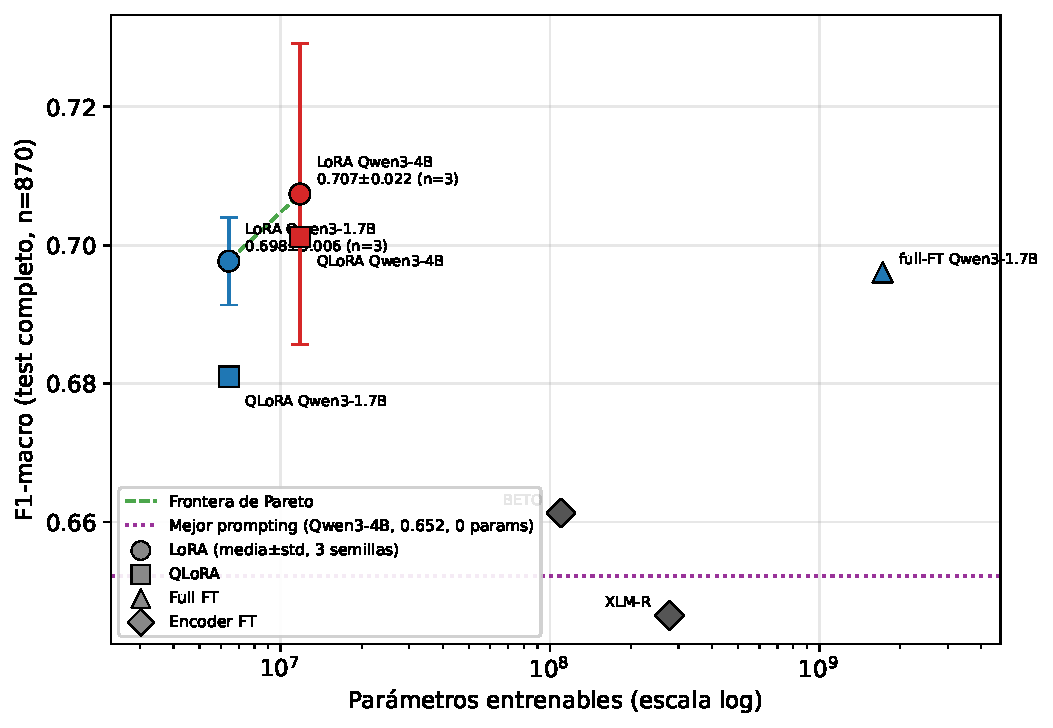
\includegraphics[width=\columnwidth]{figB_quality_cost_paper}
  \caption{Vista de Pareto calidad frente a coste para los métodos con datos
    completos.
    El eje horizontal muestra el número de parámetros entrenables (escala log);
    el eje vertical muestra el macro-F1 en el conjunto de test Cardiff~ES.
    Las configuraciones LoRA (círculos rellenos) dominan la frontera de Pareto:
    superan a las líneas base de codificadores (BETO~0.661, XLM-R~0.646) y a la
    mejor referencia de prompting (Qwen3-4B $k=4$, 0.652) con
    $17$--$43\times$ (1.7B) y $9$--$24\times$ (4B) menos parámetros entrenables
    que los codificadores.
    Las variantes QLoRA (círculos vacíos) cambian una pequeña reducción de F1 por
    una reducción de VRAM de $1.8$--$2.5\times$.
    El ajuste fino completo de Qwen3-1.7B (triángulo) iguala la calidad de LoRA
    con $\approx\!268\times$ el número de parámetros.}
  \label{fig:cutB}
\end{figure}

\begin{figure}[t]
  \centering
  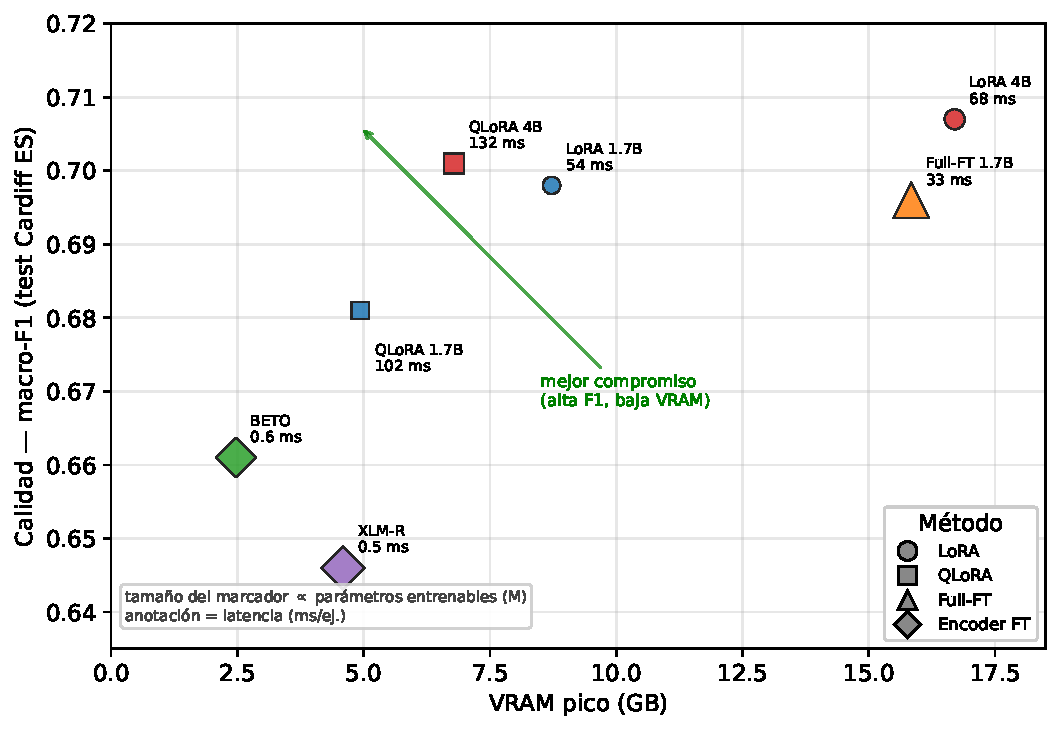
\includegraphics[width=\columnwidth]{figE_quality_cost_paper}
  \caption{Compromiso calidad/coste de los métodos con datos completos
    (Corte~B). El eje vertical muestra la calidad (macro-F1) y el horizontal la
    VRAM pico (GB); el tamaño del marcador es proporcional a los parámetros
    entrenables y la anotación indica la latencia de inferencia (ms/ej.).
    La esquina superior izquierda (alta calidad, baja VRAM) es la más deseable:
    QLoRA acerca los modelos a ella reduciendo la VRAM con una pérdida mínima de
    F1, mientras que el ajuste fino completo (triángulo) y los codificadores
    quedan lejos en parámetros o en calidad.
    Todas las cifras proceden de la Tabla~\ref{tab:cutB}.}
  \label{fig:cutB_cost}
\end{figure}

\subsubsection*{Análisis de errores por clase}

La Tabla~\ref{tab:perclass} desglosa el macro-F1 por clase para todos los métodos
con datos completos; la Figura~\ref{fig:perclass} lo visualiza.
La clase neutral es de forma consistente la más difícil en todos los modelos y
métodos: XLM-RoBERTa-base alcanza solo $0.500$ de F1 en neutral---equivalente a
una asignación aleatoria de clase para un problema balanceado de tres
clases---mientras que BETO mejora marginalmente hasta $0.550$.
Por el contrario, el sentimiento negativo y el positivo se recuperan con una
fidelidad considerablemente mayor por ambos codificadores ($0.702$ y
$0.702$--$0.737$ respectivamente), lo que confirma que la asimetría a nivel de
clase no es un artefacto de la arquitectura del codificador ni de la receta de
entrenamiento.

Los modelos generativos con LoRA cierran sustancialmente la brecha en neutral.
Qwen3-4B LoRA alcanza un F1 en neutral de $0.613$ (media sobre las
semillas~42--44), una ganancia de $+0.063$ sobre BETO y de $+0.113$ sobre
XLM-RoBERTa-base.
Qwen3-1.7B LoRA logra $0.631$, incluso ligeramente por encima del modelo más
grande en esta clase.
Las variantes QLoRA y de ajuste fino completo interpolan entre los valores de los
codificadores y de LoRA ($0.578$--$0.609$ en neutral), y el mismo orden---LoRA
$>$ QLoRA/Full-FT $>$ codificadores---se mantiene en cada fila de la tabla.

El orden entre clases es idéntico para todos los modelos: \textit{positivo}
$\geq$ \textit{negativo} $>$ \textit{neutral}.
Esta simetría indica que la dificultad de la clase neutral es una propiedad
intrínseca de la tarea y no un artefacto del fine-tuning.
El sentimiento neutral denota la \emph{ausencia} de señal afectiva en lugar de
una polaridad positiva: un tuit clasificado como neutral puede contener palabras
de opinión que se cancelan entre sí, lenguaje coloquial sin contenido
evaluativo, o afirmaciones puramente factuales.
Cualquier modelo---codificador o generativo---debe detectar eficazmente la
\emph{ausencia de sentimiento} en lugar de un patrón superficial distintivo, lo
que es intrínsecamente más difícil.
La ventaja de LoRA sobre los codificadores en esta clase es, por tanto,
especialmente reveladora: sugiere que el conocimiento lingüístico implícito más
rico codificado en el preentrenamiento de Qwen3 (que cubre un corpus mucho mayor
y más diverso que los 3\,GB de texto en español de BETO) proporciona señal
adicional para identificar enunciados neutrales que los modelos solo de
codificador entrenados principalmente en español no logran capturar con la misma
eficiencia.
La métrica macro-F1 da correctamente el mismo peso a esta clase más difícil, lo
que la convierte en la cifra única más informativa para comparar la calidad de
los sistemas en este benchmark.

\begin{table}[t]
  \centering
  \caption{F1 por clase en el conjunto de test Cardiff~ES (870 ej.).
    Resultados de LoRA: media\,$\pm$\,desv.\ típica sobre las semillas
    \{42,43,44\}; el resto: semilla~42.
    La clase neutral es de forma consistente la más débil en todos los modelos y
    métodos.}
  \label{tab:perclass}
  \small
  \resizebox{\columnwidth}{!}{%
  \begin{tabular}{@{}llrrr@{}}
    \toprule
    Modelo & Método & F1-neg & F1-neu & F1-pos \\
    \midrule
    Qwen3-4B   & LoRA   & $0.746 \pm 0.029$ & $0.613 \pm 0.023$ & $0.764 \pm 0.021$ \\
    Qwen3-4B   & QLoRA  & $0.747$           & $0.609$           & $0.748$ \\
    Qwen3-1.7B & LoRA   & $0.731 \pm 0.012$ & $0.631 \pm 0.014$ & $0.731 \pm 0.013$ \\
    Qwen3-1.7B & QLoRA  & $0.731$           & $0.578$           & $0.734$ \\
    Qwen3-1.7B & Full-FT & $0.745$          & $0.600$           & $0.744$ \\
    \midrule
    BETO        & Full-FT & $0.702$          & $0.550$           & $0.732$ \\
    XLM-R-base  & Full-FT & $0.702$          & $0.500$           & $0.737$ \\
    \bottomrule
  \end{tabular}}
\end{table}

\begin{figure}[t]
  \centering
  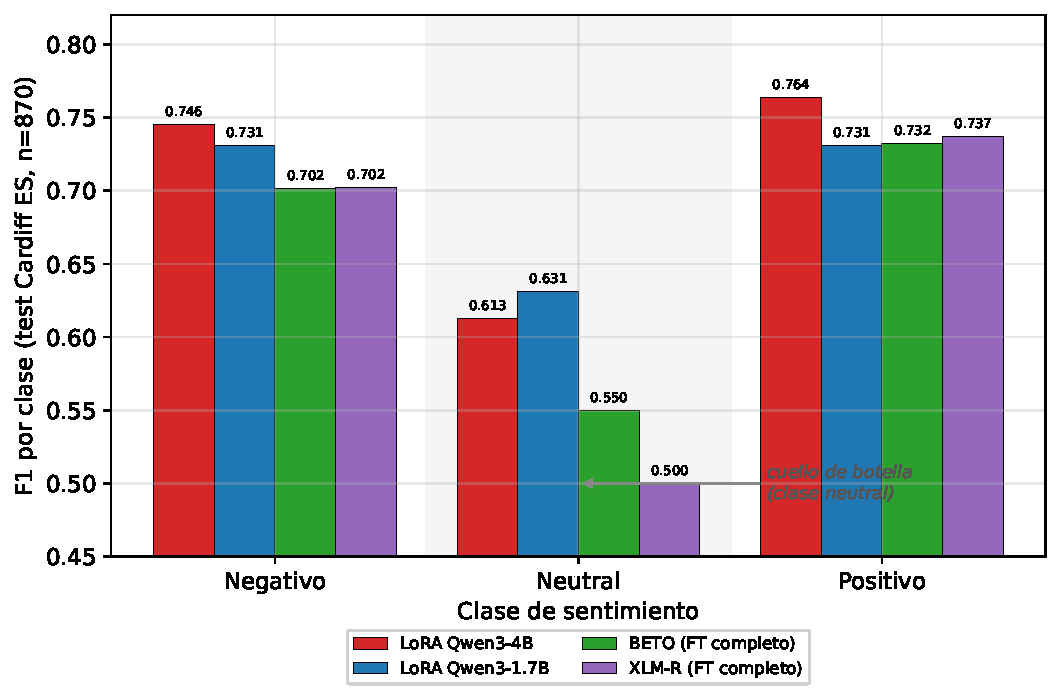
\includegraphics[width=\columnwidth]{figD_per_class_paper}
  \caption{F1 por clase (negativo, neutral, positivo) en el conjunto de test
    Cardiff~ES para LoRA Qwen3-4B, LoRA Qwen3-1.7B, BETO y XLM-R
    (resultados de LoRA: media sobre 3 semillas \{42,43,44\}).
    La clase neutral es el cuello de botella para los cuatro sistemas: los
    codificadores caen hasta 0.500--0.550, mientras que LoRA la sostiene en torno
    a 0.61--0.63. Los valores coinciden con la Tabla~\ref{tab:perclass}.}
  \label{fig:perclass}
\end{figure}

% ---- IV-C. Cut C: Dialectal Transfer ----
\subsection{Corte C: transferencia dialectal entre variedades del español}
\label{sec:results_C}

\subsubsection*{Corpus y configuración}

El Corte~C usa tres variedades nacionales extraídas de la pista
InterTASS 2018~\cite{martinezcamara2018tass}:
español ibérico (ES), español costarricense (CR) y español peruano (PE).
Las anotaciones originales de InterTASS usan cuatro polaridades
(\textit{P}, \textit{N}, \textit{NEU}, \textit{NONE}).
Las mapeamos a tres clases: \textit{positivo} (P),
\textit{negativo} (N) y \textit{neutral} (NEU).
La etiqueta \textit{NONE} (``sin opinión expresada'') se descarta: fusionarla
con \textit{neutral} contaminaría el esquema de polaridad porque NONE
denota la ausencia de un objetivo en lugar de una postura neutral, una categoría
conceptualmente distinta.
Tras descartar NONE, los conjuntos de entrenamiento utilizables contienen
\textbf{738~ES / 539~CR / 541~PE} ejemplos; una partición reservada estratificada
del 15\% de cada conjunto de entrenamiento (131~ES / 96~CR / 96~PE) se reserva
para la selección de checkpoint (mejor macro-F1 de validación, protocolo idéntico
al del Corte~B).
La evaluación se realiza sobre las respectivas particiones de \emph{desarrollo}
de InterTASS 2018 (444~ES / 242~CR / 262~PE).

Es necesaria una nota metodológica sobre las particiones de evaluación.
Las etiquetas de oro del test de InterTASS 2018 se distribuyen como un fichero
\texttt{.qrel} que devolvió HTTP~404 en el momento de redactar este trabajo; por
tanto, el conjunto de test es inaccesible.
Reportamos todos los resultados del Corte~C sobre las particiones de desarrollo
de InterTASS.
Esta es una decisión metodológica honesta, no una elección de modelado: la
partición de desarrollo no se usó durante el entrenamiento ni en la selección de
checkpoint (que usó el 15\% reservado de los datos de entrenamiento descrito
arriba), por lo que sigue siendo un conjunto de evaluación reservado.
No obstante, los lectores deben tener en cuenta que los resultados sobre la
partición de desarrollo no pueden compararse directamente con sistemas que
evaluaron sobre el conjunto de test de InterTASS.

La clase neutral es sustancialmente más prevalente en el español peruano
(PE~$\approx$~26\%) que en las otras dos variedades
(ES~$\approx$~15\%, CR~$\approx$~15\%), lo que crea una distribución más
desbalanceada que el corpus Cardiff~ES usado en los Cortes~A--B
(33\% por clase, perfectamente balanceado).

\subsubsection*{Diseño de la matriz de transferencia}

Entrenamos adaptadores LoRA sobre la partición de entrenamiento completa de cada
variedad de origen y evaluamos sobre la partición de desarrollo de cada variedad
objetivo, produciendo una matriz de transferencia de $3 \times 3$ por modelo.
Las entradas de la diagonal (entrenar y evaluar en la misma variedad) representan
el rendimiento en dominio; las entradas fuera de la diagonal miden la
transferencia entre variedades.
Tanto Qwen3-1.7B como Qwen3-4B se evalúan con los mismos hiperparámetros de LoRA
que en el Corte~B ($r=16$, lr~$=2\times10^{-4}$, 5~épocas,
min\_steps~$=80$, semillas~$\{42,43,44\}$).
El arnés generativo (parseo + reserva neutral) es idéntico al de los
Cortes~A--B; la tasa de reserva es 0.0 en las 54 celdas evaluadas.

\subsubsection*{Resultados}

La Tabla~\ref{tab:cutC} reporta el macro-F1 medio $\pm$ desviación típica sobre
tres semillas para cada combinación (variedad de origen, variedad objetivo,
modelo).
La Figura~\ref{fig:cutC} visualiza las dos matrices de $3\times3$ como mapas de
calor, con la diagonal (techo en dominio) resaltada.

\begin{table}[t]
  \centering
  \caption{Corte~C: macro-F1 de la matriz de transferencia (media\,$\pm$\,desv.\
    típica sobre las semillas \{42,43,44\}) en las particiones de desarrollo de
    InterTASS~2018.
    Filas = variedad de entrenamiento; columnas = variedad de evaluación.
    Las entradas de la diagonal (techo en dominio) están en \textbf{negrita}.
    Evaluado sobre las particiones de desarrollo debido a la inaccesibilidad de
    las etiquetas de oro del test de InterTASS~2018.}
  \label{tab:cutC}
  \small
  \resizebox{\columnwidth}{!}{%
  \begin{tabular}{@{}llrrr@{}}
    \toprule
    Modelo & Entren.$\backslash$Eval & ES-dev & CR-dev & PE-dev \\
    \midrule
    \multirow{3}{*}{Qwen3-1.7B}
      & ES  & $\mathbf{0.644\!\pm\!0.007}$ & $0.684\!\pm\!0.026$ & $0.663\!\pm\!0.031$ \\
      & CR  & $0.613\!\pm\!0.007$ & $\mathbf{0.682\!\pm\!0.023}$ & $0.631\!\pm\!0.009$ \\
      & PE  & $0.613\!\pm\!0.008$ & $0.688\!\pm\!0.005$ & $\mathbf{0.670\!\pm\!0.010}$ \\
    \midrule
    \multirow{3}{*}{Qwen3-4B}
      & ES  & $\mathbf{0.687\!\pm\!0.007}$ & $0.662\!\pm\!0.015$ & $0.678\!\pm\!0.021$ \\
      & CR  & $0.655\!\pm\!0.010$ & $\mathbf{0.683\!\pm\!0.018}$ & $0.685\!\pm\!0.018$ \\
      & PE  & $0.648\!\pm\!0.015$ & $0.688\!\pm\!0.011$ & $\mathbf{0.691\!\pm\!0.014}$ \\
    \bottomrule
  \end{tabular}}
\end{table}

\begin{figure}[t]
  \centering
  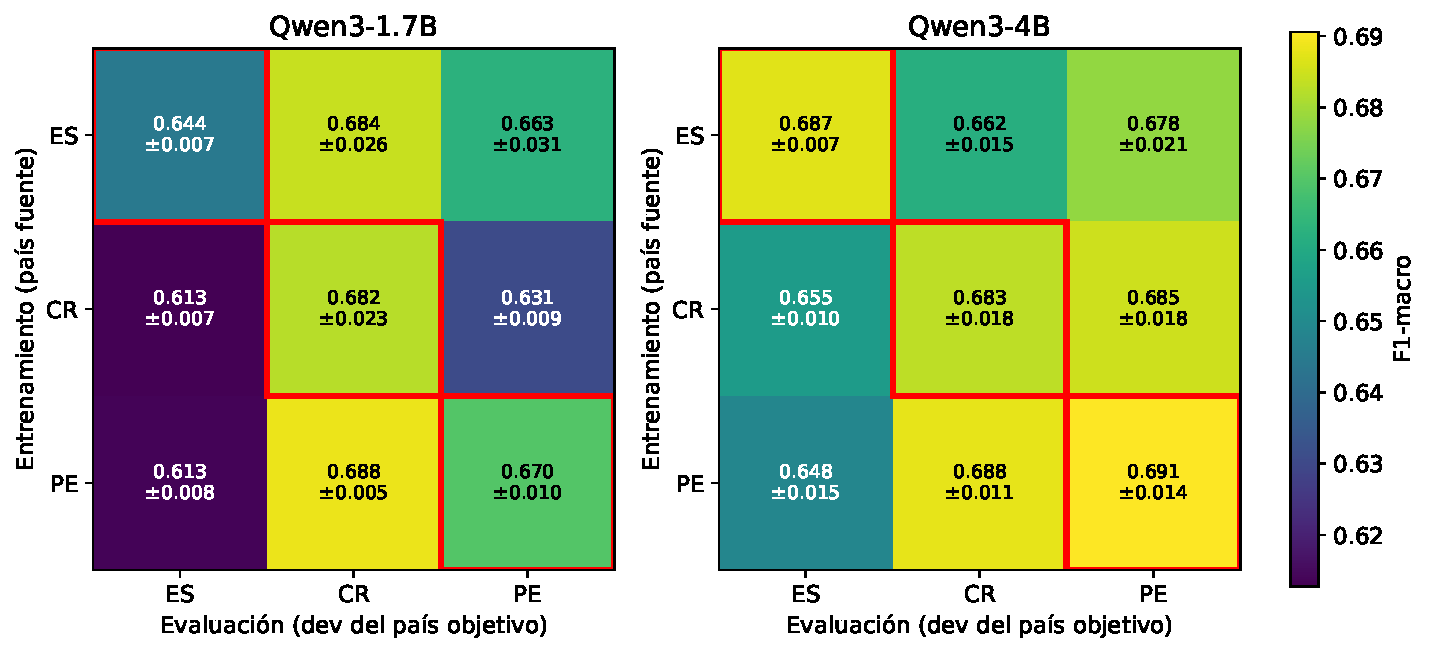
\includegraphics[width=\columnwidth]{figC_transfer_paper}
  \caption{Corte~C: matrices de transferencia dialectal para Qwen3-1.7B
    (izquierda) y Qwen3-4B (derecha). Filas = variedad de entrenamiento;
    columnas = variedad de evaluación (particiones de desarrollo de
    InterTASS~2018). El color codifica el macro-F1 (media sobre
    3 semillas); los valores se anotan como media\,$\pm$\,desv.\ típica. Las
    entradas de la diagonal (techo en dominio) están recuadradas en rojo.
    El patrón asimétrico---sin penalización en la transferencia a CR y PE, pero
    rendimiento consistentemente inferior al apuntar a ES desde otras
    variedades---es idéntico en ambos tamaños de modelo.}
  \label{fig:cutC}
\end{figure}

El hallazgo central es una \textbf{asimetría direccional en la transferencia
entre variedades}: la dirección de la transferencia importa tanto como su
magnitud.

\textbf{Sin penalización de transferencia hacia CR y PE.}
Tanto para CR-dev como para PE-dev, los adaptadores entrenados en una variedad
distinta del español rinden en la diagonal en dominio o por encima de ella.
Para Qwen3-1.7B, los adaptadores entrenados en PE y evaluados en CR-dev logran
$0.688\pm0.005$, superando el techo en dominio de CR de $0.682\pm0.023$;
los adaptadores entrenados en ES sobre PE-dev ($0.663\pm0.031$) igualan o superan
asimismo la diagonal de PE ($0.670\pm0.010$) dentro del ruido de semilla.
El mismo patrón se mantiene para Qwen3-4B: los adaptadores entrenados en CR sobre
PE-dev ($0.685\pm0.018$) igualan esencialmente el techo en dominio de PE
($0.691\pm0.014$), y los adaptadores entrenados en PE sobre CR-dev
($0.688\pm0.011$) igualan la diagonal de CR ($0.683\pm0.018$).
En ningún caso que apunte a CR o PE la brecha entre variedades supera de forma
consistente aproximadamente $1.2\sigma$ de la variabilidad a nivel de semilla.

\textbf{Penalización robusta de transferencia hacia ES (español ibérico).}
Por el contrario, entrenar en CR o PE y evaluar en ES-dev muestra un rendimiento
claramente inferior respecto a la diagonal en dominio de ES.
Para Qwen3-1.7B, CR$\rightarrow$ES produce $0.613\pm0.007$ (frente al
$0.644\pm0.007$ en dominio, una brecha de $\Delta=-0.031$) y PE$\rightarrow$ES
produce $0.613\pm0.008$ ($\Delta=-0.031$).
Expresadas en unidades de desviación típica a nivel de semilla, estas brechas
corresponden a 4.6$\sigma$ y 3.8$\sigma$ respectivamente.
Para Qwen3-4B, CR$\rightarrow$ES produce $0.655\pm0.010$
(frente a $0.687\pm0.006$, $\Delta=-0.032$, 3.1$\sigma$) y
PE$\rightarrow$ES produce $0.648\pm0.015$ ($\Delta=-0.039$, 2.6$\sigma$).
La penalización hacia ES supera, por tanto, 2$\sigma$ de la variabilidad a nivel
de semilla en las cuatro comparaciones entre variedades hacia ES---en ambos
tamaños de modelo.

Señalamos una excepción que no se replica: en Qwen3-1.7B,
la brecha CR$\rightarrow$PE es de 3.9$\sigma$ (lo que sugiere una penalización
leve), pero la cifra análoga para Qwen3-4B es de solo 0.3$\sigma$, claramente
dentro del ruido.
La columna ES es la única asimetría direccional que se replica de forma
consistente en ambos tamaños de modelo.

Es importante ser explícitos sobre la fortaleza de esta afirmación.
Estas brechas se caracterizan en términos de desviaciones típicas a nivel de
semilla---una medida de magnitud relativa al ruido observado entre semillas
aleatorias.
No se ha realizado ninguna prueba de hipótesis formal (p.\ ej.\ una prueba de
permutación o una $t$ de Student pareada), ni se ha aplicado ninguna corrección
por comparaciones múltiples a lo largo de la matriz de $3\times3\times2$.
El criterio de $2\sigma$ es una heurística de magnitud, no un umbral de
significación estadística; el lector no debe interpretar estos valores como
$p$-valores ni como evidencia de significación en el sentido clásico de las
pruebas de hipótesis.
Dados los tamaños pequeños de los corpus (menos de 740 ejemplos de entrenamiento
por variedad) y tres semillas, los resultados son sugerentes pero se
beneficiarían de una replicación en corpus más grandes con pruebas estadísticas
formales.

\textbf{La escala no cambia el patrón; eleva el techo.}
Qwen3-4B eleva uniformemente el techo de macro-F1 en 2--4 puntos porcentuales
(en dominio: ES 0.687 frente a 0.644; CR 0.683 frente a 0.682; PE 0.691 frente a
0.670), pero la asimetría direccional---sin penalización a CR/PE, penalización
consistente a ES---es idéntica en las matrices de 1.7B y 4B.
Por tanto, el patrón no es un artefacto de la capacidad del modelo.

% ============================================================
%  V. DISCUSSION
% ============================================================

\section{Discusión}
\label{sec:discussion}

Los resultados de la Sección~\ref{sec:results} responden a las tres preguntas
de investigación planteadas en la Introducción, pero las cifras por sí solas no
reflejan toda su relevancia práctica.
Esta sección interpreta qué significan el patrón del punto de cruce y la
frontera de Pareto para los profesionales, y sitúa los hallazgos dentro de las
limitaciones del diseño experimental.

\subsubsection*{Por qué el punto de cruce se desplaza con el tamaño del modelo}

La observación central del Corte~A---que Qwen3-1.7B necesita menos de diez
ejemplos etiquetados para superar su propio mejor resultado de prompting,
mientras que Qwen3-4B requiere aproximadamente cincuenta---se deriva
directamente del mecanismo descrito por
Min et al.~\cite{min2022rethinking}: las demostraciones en contexto comunican
principalmente el formato y el espacio de etiquetas, de modo que el techo de
calidad del prompting está gobernado por el conocimiento preentrenado del
modelo.
Un modelo más grande y con mejor seguimiento de instrucciones ya codifica un
conocimiento previo más preciso sobre el sentimiento en español, lo que eleva
su suelo de prompting (0.652 frente a 0.560 de mejor F1 few-shot).
El fine-tuning con LoRA debe superar ese suelo antes de aportar una ganancia
neta de calidad; lograrlo exige proporcionalmente más señal etiquetada.

Este desplazamiento dependiente del tamaño matiza la heurística habitual entre
profesionales de que ``el fine-tuning siempre gana con suficientes datos''.
La regla más precisa es que \emph{el umbral de datos a partir del cual el
fine-tuning resulta preferible escala con la calidad de prompting del modelo
base}.
Un profesional con muy pocas etiquetas ($n < 10$) y un modelo pequeño (1--2B)
debería ajustar de inmediato; ese mismo profesional con un modelo de 4B debería
evaluar primero si el suelo de prompting ya alcanza su objetivo de calidad,
dado que el fine-tuning solo se vuelve fiablemente superior en torno a
$n \approx 50$ en nuestro escenario.

\subsubsection*{Implicaciones de la frontera de Pareto para despliegues con presupuesto limitado}

Las configuraciones LoRA se sitúan estrictamente por encima de la frontera de
Pareto calidad-coste respecto a las líneas base de codificadores.
Qwen3-4B LoRA (F1\,=\,0.707, 11.8\,M de parámetros entrenables) y Qwen3-1.7B
LoRA (F1\,=\,0.698, 6.4\,M de parámetros) superan ambos al mejor codificador
controlado, BETO (F1\,=\,0.661, 110\,M de parámetros actualizados), por 4--6
puntos porcentuales, entrenando aproximadamente entre $9$ y $17\times$ menos
parámetros que BETO.
Para profesionales en entornos con presupuesto restringido---donde el
almacenamiento de adaptadores y el coste de reentrenamiento por tarea son las
restricciones vinculantes---esta dominancia es decisiva: no existe escenario en
el que un ajuste fino completo de un codificador sea preferible a LoRA en los
ejes calidad-coste que medimos.

El ajuste fino completo de Qwen3-1.7B (F1\,=\,0.696) es la ilustración más clara
de este punto: iguala la calidad de LoRA solo en un decimal, mientras consume
$\approx\!268\times$ más parámetros entrenables y casi el doble de VRAM
(15.84\,GB frente a 8.72\,GB).
La única ventaja del ajuste fino completo es la latencia de inferencia
(33\,ms/ej.\ frente a 54\,ms/ej.), atribuible a la ausencia de sobrecoste de
adaptadores durante la decodificación.
Para el procesamiento por lotes en diferido esta ventaja puede ser irrelevante;
para una API en tiempo real puede importar.
En todos los demás aspectos, el ajuste fino completo queda dominado.

Merece comentario que RoBERTuito (0.758, Tabla~\ref{tab:baselines}) supere a
todas las configuraciones controladas de este estudio.
Este resultado no contradice nuestras conclusiones: RoBERTuito fue ajustado
sobre TASS~2020, un corpus de tuits en español con una tarea idéntica, por lo
que su evaluación ``lista para usar'' sobre Cardiff~ES constituye una
transferencia desde un dominio muy cercano y no una comparación controlada del
coste de adaptación---de hecho, ilustra precisamente el valor del fine-tuning
específico de tarea que este trabajo cuantifica.
Nuestra contribución no es superar a todo sistema existente, sino medir, bajo un
protocolo controlado con el mismo presupuesto de datos y cómputo, la frontera
calidad-coste de adaptar modelos generativos pequeños frente a codificadores.

\subsubsection*{El compromiso VRAM-calidad de QLoRA}

La cuantización NF4 de QLoRA reduce la VRAM pico en $1.8$--$2.5\times$ (hasta
4.93\,GB y 6.79\,GB para los modelos de 1.7B y 4B respectivamente) con una
penalización de calidad de solo 1--2.5 puntos porcentuales de F1.
No obstante, el compromiso es asimétrico entre tamaños de modelo.
Para el modelo de 4B, QLoRA retiene el 99.2\% del F1 de LoRA a 6.79\,GB---lo que
sitúa el modelo dentro del presupuesto de las GPU de consumo de 8\,GB
(RTX~3070, RTX~4060~Ti), a diferencia de la gama empresarial H200/A100.
Este es un resultado genuinamente habilitador: un profesional sin acceso a
hardware empresarial en la nube puede desplegar un clasificador competitivo de
sentimiento en español por el coste de una GPU de gama media para videojuegos.
Para el modelo de 1.7B, LoRA ya cabe holgadamente en 8.72\,GB, de modo que el
ahorro de QLoRA es menos crítico en la práctica---aunque sigue siendo útil en
entornos donde varios modelos deben coexistir en el mismo dispositivo.

Los costes de QLoRA son reales y no deben pasarse por alto: el entrenamiento es
$\approx\!2.4\times$ más lento (debido a la decuantización NF4 durante el paso
hacia delante) y la latencia de inferencia es aproximadamente $2\times$ mayor.
Para el procesamiento por lotes asíncrono estas penalizaciones son tolerables;
para la inferencia de baja latencia (requisitos de tiempo de respuesta
inferiores a 100\,ms) LoRA con el modelo base sin cuantizar es la mejor opción
si la VRAM lo permite.

\subsubsection*{Revisión de las preguntas de investigación}

Retomamos las tres preguntas planteadas en la Sección~\ref{sec:introduction}.

\textbf{(1) ¿Cuándo supera el fine-tuning con PEFT al prompting del mismo
modelo?}
La respuesta depende del tamaño del modelo: para Qwen3-1.7B el punto de cruce se
produce entre $n=4$ y $n=7$ ejemplos etiquetados; para Qwen3-4B se difiere hasta
aproximadamente $n=50$.
Ninguno de estos umbrales es una constante universal---ambos son funciones del
propio suelo de prompting del modelo y, probablemente, de la tarea y el dominio.
Será necesario trabajo futuro con distintos modelos y tareas para generalizar
este hallazgo, pero la existencia de un desplazamiento dependiente del tamaño es
en sí misma un resultado reproducible y prácticamente accionable.

\textbf{(2) ¿Pueden los LLM generativos pequeños con LoRA superar a las líneas
base de codificadores en español controlando el coste?}
Sí: LoRA aplicado a Qwen3-1.7B y Qwen3-4B supera a BETO y
XLM-RoBERTa-base por 4--6 puntos de F1 con entre $17$ y $43\times$ menos
parámetros entrenables para el modelo de 1.7B (entre $9$ y $24\times$ para el de
4B).
Ambos resultados son reproducibles en hardware gratuito (el LoRA de 1.7B cabe
holgadamente en 8.72\,GB de VRAM; el QLoRA de 4B cabe en 6.79\,GB), lo que
confirma la accesibilidad práctica del enfoque.

\textbf{(3) ¿Transfieren sin penalización los adaptadores LoRA entrenados en una
variedad dialectal del español a otras?}
La respuesta depende de la variedad.
La transferencia a CR y PE es esencialmente gratuita: los adaptadores entre
variedades igualan el rendimiento en dominio dentro del ruido a nivel de semilla
en ambas variedades objetivo y en ambos tamaños de modelo.
Sin embargo, la transferencia al español ibérico (ES) incurre en una
penalización consistente y replicada de 0.031--0.039 puntos de macro-F1,
caracterizada como 2.6--4.6$\sigma$ de la variabilidad a nivel de semilla
(véase la Sección~\ref{sec:results_C} para las salvedades completas sobre esta
caracterización).
La implicación práctica es que un profesional que despliegue un único adaptador
de sentimiento en español entre variedades debería priorizar CR o PE---donde los
adaptadores fuera de dominio rinden a la par que los de dominio---y debería
recopilar al menos algunos datos de entrenamiento específicos del español
ibérico antes de apuntar a ES, o bien recurrir directamente a adaptadores
entrenados en ES.

\subsubsection*{Amenazas a la validez}

Las principales limitaciones de este estudio se enumeran en detalle en la
Sección~\ref{sec:conclusions}.
En síntesis: los Cortes~A y~B se apoyan en un único corpus de Twitter
(Cardiff~ES); el Corte~C usa particiones de desarrollo de InterTASS~2018 y
corpus de tamaño moderado por variedad; y los tiempos de entrenamiento proceden
de una NVIDIA H200, por lo que diferirán en hardware T4 real.
Estas restricciones no invalidan los hallazgos centrales, pero aconsejan cautela
al extrapolar los umbrales numéricos a dominios o tareas sustancialmente distintos.

% ============================================================
%  VI. CONCLUSIONS AND FUTURE WORK
% ============================================================

\section{Conclusiones y trabajo futuro}
\label{sec:conclusions}

Este artículo presenta un estudio empírico reproducible de LoRA y QLoRA
aplicados a LLM generativos pequeños de pesos abiertos (Qwen3-1.7B y Qwen3-4B,
1--4B parámetros) para el análisis de sentimiento de tuits en español en tres
clases, realizado bajo restricciones de GPU de capa gratuita (objetivo de
despliegue T4 16~GB).
Abordamos tres preguntas de investigación---cuándo compensa el fine-tuning con
PEFT frente al prompting del mismo modelo; pueden los LLM generativos pequeños
con LoRA dominar a las líneas base de codificadores establecidas en español en
la frontera calidad-coste; y transfieren sin penalización los adaptadores LoRA
entrenados en una variedad dialectal del español a otras---y damos respuestas
empíricamente fundamentadas a las tres.

\textbf{Hallazgo 1 (Corte~A): el punto de cruce de prompting a fine-tuning
depende del tamaño del modelo, no es universal.}
Para Qwen3-1.7B, cuyo mejor resultado de prompting few-shot es F1\,=\,0.560
($k=8$), LoRA supera ese listón con tan solo $n=7$ ejemplos etiquetados
($0.590 \pm 0.063$), lo que significa que menos de diez tuits anotados bastan
para justificar el fine-tuning frente al aprendizaje en contexto.
Para Qwen3-4B, cuyo suelo de prompting más fuerte alcanza F1\,=\,0.652 ($k=4$),
el punto de cruce se difiere hasta aproximadamente $n=50$
($0.666 \pm 0.034$)---aproximadamente un orden de magnitud más de datos que los
requeridos por el modelo más pequeño.
El mecanismo es claro: un suelo de prompting más alto exige más señal de
fine-tuning para superarlo.
Este desplazamiento dependiente del tamaño es el hallazgo empírico central del
Corte~A y tiene implicaciones prácticas directas: los profesionales con muy pocas
etiquetas (digamos $n < 10$) deberían elegir el modelo capaz más pequeño para el
fine-tuning, mientras que quienes dispongan de presupuestos moderados
($n \approx 50$--$100$) se beneficiarán del mayor techo de calidad del modelo de
4B.

\textbf{Hallazgo 2 (Corte~B): LoRA domina la frontera de Pareto calidad-coste.}
Con datos de entrenamiento completos, las configuraciones LoRA superan a la mejor
línea base de codificador controlado (BETO~0.661) actualizando solo 6--12~M de
parámetros.
Qwen3-4B LoRA logra F1\,=\,$0.707 \pm 0.022$ y Qwen3-1.7B LoRA logra
F1\,=\,$0.698 \pm 0.006$, ganancias de 4--6 puntos porcentuales sobre BETO y
XLM-RoBERTa-base (0.646) con aproximadamente $17$--$43\times$ menos parámetros
entrenables para el modelo de 1.7B ($9$--$24\times$ para el de 4B).
El ajuste fino completo de Qwen3-1.7B (F1\,=\,0.696, 1.72B parámetros entrenables)
queda dominado por LoRA en todos los ejes relevantes excepto la latencia de
inferencia.
QLoRA retiene el 97--99\% del F1 de LoRA con una VRAM pico 1.8--2.5$\times$ menor
(4.93~GB para 1.7B; 6.79~GB para 4B), lo que hace accesibles los modelos de 4B en
hardware de consumo de 8~GB a costa de un mayor tiempo de entrenamiento y
latencia de inferencia.

\textbf{Hallazgo 3 (Corte~C): la transferencia dialectal es asimétrica, siendo el
español ibérico la variedad objetivo más sensible.}
Un experimento de transferencia entre variedades de $3\times3$ sobre
InterTASS~2018 revela que los adaptadores LoRA transfieren libremente entre
variedades en la mayoría de las direcciones: los adaptadores entrenados en CR o
PE igualan el rendimiento en dominio sobre CR-dev y PE-dev, con brechas entre
variedades consistentemente dentro de $\approx1.2\sigma$ del ruido a nivel de
semilla.
La excepción notable es el español ibérico como objetivo de evaluación:
entrenar en CR o PE y evaluar en ES-dev incurre en una penalización de macro-F1
de 0.031--0.039 puntos (2.6--4.6$\sigma$ de la variabilidad a nivel de semilla)
que se replica de forma idéntica en Qwen3-1.7B y Qwen3-4B.
Escalar de 1.7B a 4B eleva el techo de macro-F1 en 2--4 puntos de forma uniforme,
pero no altera la asimetría direccional.
Este hallazgo se caracteriza por su magnitud relativa al ruido a nivel de
semilla; no se ha realizado ninguna prueba estadística formal, y se recomienda
una replicación en corpus más grandes con pruebas formales antes de hacer
afirmaciones causales fuertes.

\textbf{Limitaciones.}
Varios aspectos de este estudio aconsejan cautela al generalizar sus
conclusiones:

\begin{itemize}
  \item \emph{Un único conjunto de datos.} Todos los resultados proceden del
    corpus Cardiff~ES (sentimiento de tuits, tres clases, particiones
    balanceadas).
    No se ha comprobado la generalización a otros dominios---noticias, reseñas,
    atención al cliente---ni a otras formulaciones de tarea.

  \item \emph{Particularidades del dominio de Twitter.} Los tuits son cortos,
    ruidosos e informales; los hallazgos pueden no transferirse a textos más
    largos o más formales sin validación adicional.

  \item \emph{Varianza de semilla (Corte~B).} La mayoría de las condiciones del
    Corte~B usan una única semilla (42); la varianza de semilla documentada para
    las condiciones de LoRA con datos completos es baja ($\pm0.006$ para 1.7B,
    $\pm0.022$ para 4B) pero no se elimina.

  \item \emph{Discrepancia de hardware.} Los experimentos se ejecutaron en GPU
    NVIDIA H200.
    El uso de VRAM se monitorizó por celda para validar la viabilidad en
    T4 16~GB, pero los tiempos de ejecución del entrenamiento diferirán en
    hardware T4 real.

  \item \emph{Corte~C: corpus pequeños y desbalanceo de clases.}
    InterTASS~2018 proporciona solo 539--738 ejemplos de entrenamiento por
    variedad tras eliminar NONE.
    Los corpus pequeños pueden causar infraentrenamiento respecto a Cardiff~ES
    (1,839 ejemplos), y la clase neutral es particularmente escasa (15\% en
    ES y CR; 26\% en PE), lo que conduce a un F1 menor en la clase neutral y a
    una mayor varianza entre semillas que en los Cortes~A--B.
    La etiqueta neutral en InterTASS es además inherentemente ambigua, ya que
    puede confundirse con ambas clases polares en modelos que carecen de
    suficiente señal dialectal.

  \item \emph{Corte~C: cobertura dialectal limitada.}
    Los resultados cubren solo tres de las muchas variedades dialectales del
    español (ES, CR, PE).
    Las generalizaciones a otras variedades---mexicana, venezolana, argentina,
    rioplatense---no están empíricamente respaldadas por este estudio.

  \item \emph{Corte~C: evaluación sobre la partición de desarrollo.}
    Todos los resultados del Corte~C usan las particiones de desarrollo de
    InterTASS~2018 porque las etiquetas de oro del test eran inaccesibles
    (HTTP~404).
    Las cifras de la partición de desarrollo no pueden compararse directamente
    con los resultados publicados sobre el conjunto de test de InterTASS.

  \item \emph{Corte~C: sin prueba estadística formal.}
    La asimetría direccional hacia ES se caracteriza por su magnitud relativa a
    las desviaciones típicas a nivel de semilla (criterio de $2\sigma$).
    No se ha aplicado ninguna prueba de hipótesis ni corrección por comparaciones
    múltiples a lo largo de la matriz de $3\times3\times2$; el criterio no debe
    interpretarse como significación estadística clásica.
\end{itemize}

\textbf{Trabajo futuro.}

\begin{itemize}
  \item \textbf{Cobertura dialectal más amplia.}
    El Corte~C cubre solo tres variedades (ES, CR, PE) de InterTASS~2018.
    Extender la matriz de transferencia al español mexicano, venezolano,
    argentino y rioplatense---y evaluar sobre particiones de test adecuadas una
    vez que las etiquetas de oro de InterTASS sean accesibles---comprobaría si la
    asimetría hacia el español ibérico se generaliza y si surgen otras
    sensibilidades específicas de variedad.
    También se necesita una prueba de hipótesis formal con corrección por
    comparaciones múltiples a lo largo de la matriz completa antes de poder hacer
    afirmaciones causales sobre la dificultad dialectal.

  \item \textbf{Modelos más grandes con QLoRA.} Extender la curva de escalado a
    modelos de 8B con QLoRA comprobaría si el patrón del punto de cruce y la
    dominancia de Pareto de LoRA se mantienen a mayor capacidad, dentro del mismo
    presupuesto de VRAM de capa gratuita mediante cuantización de 4 bits.

  \item \textbf{Panorama PEFT más amplio.} DoRA~\cite{liu2022dora} e IA$^3$
    son alternativas prometedoras que podrían extender la frontera de Pareto
    identificada en el Corte~B, ofreciendo potencialmente mejores compromisos de
    calidad por parámetro.

  \item \textbf{Otras tareas de PLN en español.} Aplicar el mismo protocolo de
    benchmarking con LoRA/QLoRA a la detección de discurso de odio y al
    reconocimiento de entidades nombradas en texto de redes sociales en español
    comprobaría la generalidad de nuestros hallazgos más allá del análisis de
    sentimiento.

  \item Un análisis complementario de robustez frente a perturbaciones típicas
    de redes sociales (mayúsculas, elongaciones, emojis, etc.) apunta a una
    fragilidad diferencial de los codificadores \textit{cased} frente a los
    modelos generativos, cuya caracterización completa se deja como extensión.

\end{itemize}

% ============================================================
%  REFERENCES
% ============================================================

\bibliographystyle{IEEEtran}
\bibliography{../docs/research/references}

% ============================================================
%  END
% ============================================================

\end{document}
